\documentclass[a4paper,11pt,titlepage]{article}
\usepackage[english]{babel}
\usepackage[utf8]{inputenc}
\usepackage[T1]{fontenc}
\usepackage[a4paper,top=1in,left=1in,right=1in,bottom=1in,marginparwidth=1.75cm]{geometry}
\usepackage{pgfplots}
\pgfplotsset{compat=1.18}
\usepackage{afterpage}
\usepackage{amsmath}
\usepackage{amsthm}
\usepackage{amssymb}
\usepackage{csquotes}
\usepackage{graphicx}
\usepackage{booktabs}
\usepackage{listings}
\lstset{frame=single,framexleftmargin=15pt}
\usepackage{caption}
\DeclareUnicodeCharacter{0302}{\^{}}
\captionsetup[figure]{labelfont={bf},labelsep=quad}
\usepackage[ruled,vlined]{algorithm2e}
\makeatletter
\DeclareMathOperator*{\argmin}{argmin}
\renewcommand{\SetKwInOut}[2]{\sbox\algocf@inoutbox{\KwSty{#2}\algocf@typo:}\expandafter\ifx\csname InOutSizeDefined\endcsname\relax\newcommand\InOutSizeDefined{}\setlength{\inoutsize}{\wd\algocf@inoutbox}\sbox\algocf@inoutbox{\parbox[t]{\inoutsize}{\KwSty{#2}\algocf@typo:\hfill}~}\setlength{\inoutindent}{\wd\algocf@inoutbox}\else\ifdim\wd\algocf@inoutbox>\inoutsize\setlength{\inoutsize}{\wd\algocf@inoutbox}\sbox\algocf@inoutbox{\parbox[t]{\inoutsize}{\KwSty{#2}\algocf@typo:\hfill}~}\setlength{\inoutindent}{\wd\algocf@inoutbox}\fi\fi\algocf@newcommand{#1}[1]{\ifthenelse{\boolean{algocf@inoutnumbered}}{\relax}{\everypar={\relax}}{\let\\\algocf@newinout\hangindent=\inoutindent\hangafter=1\parbox[t]{\inoutsize}{\KwSty{#2}\algocf@typo:\hfill}~##1\par}\algocf@linesnumbered}}
\makeatother
\usepackage{bm}
\usepackage[normalem]{ulem}
\setlength{\marginparwidth}{2cm}
\usepackage[colorinlistoftodos]{todonotes}
\usepackage[colorlinks=true, allcolors=blue]{hyperref}
\pdfstringdefDisableCommands{\def\({}\def\){}\def\theta{theta}}
\renewcommand*{\rmdefault}{bch}
\renewcommand*{\ttdefault}{lmtt}
\newcommand{\citationneeded}{\textcolor{red}{[citation-needed]}}
\setlength{\parskip}{0.5em}
\usepackage[numbers,comma,square,sort&compress]{natbib}
\bibliographystyle{abbrvunsrtnat.bst}
\theoremstyle{definition}
\newtheorem{definition}{Definition}[section]
\theoremstyle{plain}
\newtheorem{theorem}{Theorem}[section]
\newtheorem{corollary}{Corollary}[theorem]
\newtheorem{lemma}[theorem]{Lemma}
\theoremstyle{remark}
\newtheorem*{remark}{Remark}
\newcommand{\reporttitle}{Scientific Machine Learning: Neural Networks and Neural Differential Equations}
\newcommand{\reportauthorA}{Jiaru (Eric) Li (CID: 02216531)}
\newcommand{\reportauthorB}{James Tay (CID: 02015786)}
\newcommand{\reportauthorC}{Xinyan Wang (CID: 02205857)}
\newcommand{\reportauthorD}{Jiankuan Liu (CID: 02215415)}
\newcommand{\reportauthorE}{Tianshi Liu (CID: 02218664)}
\newcommand{\supervisor}{Sheehan Olver}
\begin{document}
\begin{titlepage}
\newcommand{\HRule}{\rule{\linewidth}{0.5mm}}
\begin{figure}[h]
  
\includegraphics[width=8cm]{figures/Imperial_logo.png}
  \vspace{1cm}
\end{figure}
\center
\textsc{\LARGE Imperial College London}\\[0.5cm] 
\textsc{\Large Department of Mathematics}\\[1.5cm] 
\textsc{\Large Second-year Group Research Project}\\[0.5cm]
\makeatletter
\HRule\\[0.6cm]
{\huge\bfseries\reporttitle}\\[0.6cm]
\HRule\\[1.5cm]
\begin{minipage}{0.4\textwidth}
\begin{flushleft}\large
\emph{Authors:}\\
\reportauthorA\\
\reportauthorB\\
\reportauthorC\\
\reportauthorD\\
\reportauthorE
\end{flushleft}
\end{minipage}
\begin{minipage}{0.4\textwidth}
\begin{flushright}\large
\emph{Supervisor:}\\
\supervisor
\end{flushright}
\end{minipage}\\[2cm]
\makeatother
\vfill
\makeatletter
{\large\today}\\[2cm]
\makeatother
\end{titlepage}

\begin{abstract}

This report delves into the integration of neural networks with differential equations, known as neural differential equations, within the field of scientific machine learning. They offer a continuous-time model that is particularly effective for handling time series data, surpassing traditional methods that operate in discrete time. We explore the core principles of neural networks, their architecture, and training techniques, and then introduce neural ordinary differential equations, highlighting their formulation and practical applications. As an extension, we briefly discuss neural controlled differential equations. This study not only highlights the theoretical importance of neural differential equations but also showcases their potential in various applications as part of larger neural networks.

\end{abstract}
\tableofcontents
\pagebreak
\section{Introduction}
\textcolor{red}{We will need to rewrite some sections because of moving around of content.}

In recent years, the intersection of machine learning and scientific computing has given rise to a novel field known as scientific machine learning. It takes advantage of the power of both disciplines to address complex problems that might be difficult to solve using conventional methods. A particularly exciting development in this area is the concept of neural differential equations, integrating neural networks with differential equations \cite{chen2018neural}.

The motivation behind neural differential equations stems from the limitations of traditional neural networks, such as their inability to handle continuous time series data. Neural differential equations address these issues by providing a continuous-time analogue to discrete-layer architectures such as residual neural networks. \citationneeded

In this report, we are first going to describe some foundational notions of neural networks. We begin by reviewing the history and basic structure of neural networks, including key concepts such as layers, activation functions, and training methodologies in Section \ref{sec:neuralnetworks}. We then explore some simple applications to further illustrate these ideas and help us to discover how neural networks work in terms of real-world scenarios, such as regression and classification in Section \ref{sec:neuralnetworks}.

Subsequently, we dive into the formulation and implementation of neural ODEs and mention their connection to residual neural networks in Section \ref{sec:intro}. Backpropagation and the adjoint method will be discussed in detail, and we will also show the strengths and limitations of neural ODEs in Section \ref{sec:intro}.

Furthermore, we examine the techniques for solving neural ODEs, introducing theories such as loss functions and gradient descent. We also present and analyse numerical ODE solvers, including Euler's method and Runge-Kutta methods in Section \citationneeded.

As an application, we apply neural ODEs to the MNIST handwritten digit classification task, improving the accuracy from $80\%$ achieved by the traditional neural network method to around $95\%$, thereby demonstrating the capabilities of neural ODEs in Section \ref{sec:app}.

Finally, building on the framework of neural ODEs to handle more complex and irregular data streams, we extend our discussion to neural CDEs in Section \ref{sec:extension}.

Throughout this report, we will be using the Julia programming language. This is a modern, compiled, high-level, open-source language developed at MIT. It is becoming increasingly important in scientific machine learning and is widely used in high-performance computing and artificial intelligence, including by Astrazeneca, Moderna, and Pfizer in drug development and clinical trial acceleration, IBM for medical diagnosis, MIT for robot locomotion, and elsewhere \cite{SciMLSANUM2024}. Where appropriate, we will supplement suitable Julia code to accompany the ideas.

In conclusion, we aim to provide a thorough understanding of neural differential equations and their significance in scientific machine learning.

\pagebreak
\section{Neural Networks}
\label{sec:neuralnetworks}
\subsection{History}

Before diving into neural ordinary and control differential equations, we shall first explore classic neural networks. Generally speaking, a \textit{neural network} is a group of units called \textit{neurons} connected by signals called \textit{synapses}.

In 1943, Warren McCulloch and Walter Pitts published a seminal paper, in which they proposed the first mathematical model of an \textit{artificial neural network}, inspired by biological neural networks in animal brains \cite{McCulloch1943}. This model was named the \textit{McCulloch-Pitts neuron}, or \textit{perceptron}. In some sense, it could ‘learn’ from given data and make decisions or predictions based on some parameters. The process of optimising the choice of such parameters is called \textit{training} the neural network.

Later in 1958, Frank Rosenblatt described an implementation of perceptron in detail \cite{Rosenblatt1958}. The field of neural networks has expanded rapidly and is nowadays widely used in various fields such as machine learning and artificial intelligence. We shall explore some simple applications later.

\subsection{Concepts}

\subsubsection{Structure}

An \textit{(artificial) neural network} ((A)NN) consists of interconnected neurons, each of which can be thought of as a mathematical function. They are typically organised into \textit{layers} consisting of

\begin{itemize}
    \item an \textit{input layer} that receives the input,
    \item one or more \textit{hidden layers} that processes the data, and
    \item an \textit{output layer} that produces the output.
\end{itemize}

The number of layers is usually called the \textit{depth} of the neural network. The input and output data are usually given as real numbers. Therefore, the whole neural network can be thought of as a function $f:\mathbb{R}^m\rightarrow\mathbb{R}^n$ that takes an input vector $\mathbf{x}$ of dimension $m$ and an output vector $\mathbf{\hat{y}}$ of dimension $n$. Each connection between neurons has a \textit{weight}, and possibly a \textit{bias}, which are adjusted in the optimisation process, allowing the model to generalise to unseen data. They are usually given altogether as a \textit{weight matrix} $\mathbf{W}$ and a \textit{bias vector} $\mathbf{b}$.

\subsubsection{Activation Function}

For neural networks with multiple layers, an \textit{activation function} $\sigma$ is usually used. This is because it helps to decide whether a neuron should be ‘activated’ and introduces non-linearity into the model. The output of each neuron in a layer is therefore calculated as $\mathbf{h}_{t+1}=\sigma\left(\mathbf{W}_t\mathbf{h}_t+\mathbf{b}_t\right)$, where $\sigma$ acts element-wise, $\mathbf{h}_t$ is the output vector for layer $t$, $\mathbf{W}_t$ is the weight matrix connecting layer $t$ to layer $t+1$, and $\mathbf{b}_t$ is the bias vector for layer $t$. 

Regarding the choice of the activation function, the S-shaped \textit{sigmoid function} has some nice properties: it is bounded, differentiable with a non-negative derivative, and has exactly one point of inflection \cite{HanMoraga}. Two familiar examples of sigmoid functions are the \textit{logistic function} $\sigma(x)=1/\left(1+e^{-x}\right)$ and the hyperbolic tangent function $\sigma(x)=\tanh x$. Another commonly used activation function is the \textit{rectifier}, or \textit{rectified linear unit} (ReLU), defined as $\sigma(x)=\max(0, x)$.

\begin{figure}[htbp]
    \centering
    \begin{minipage}{0.32\textwidth}
        \centering
        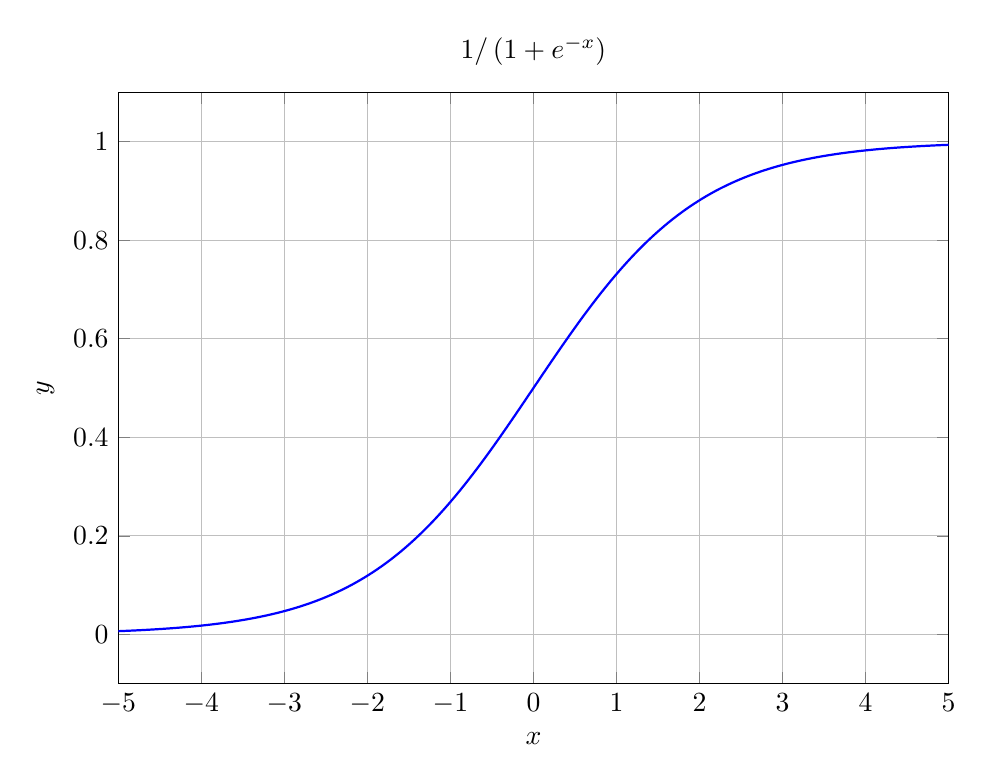
\begin{tikzpicture}
            \begin{axis}[
                title={$1/\left(1+e^{-x}\right)$},
                xlabel={$x$},
                ylabel={$y$},
                grid=major,
                width=\textwidth,
                height=0.75\textwidth,
                xmin=-5, xmax=5,
                ymin=-0.1, ymax=1.1,
            ]
                \addplot[blue, thick, samples=200] {1 / (1 + exp(-x))};
            \end{axis}
        \end{tikzpicture}
    \end{minipage}
    \hfill
    \begin{minipage}{0.32\textwidth}
        \centering
        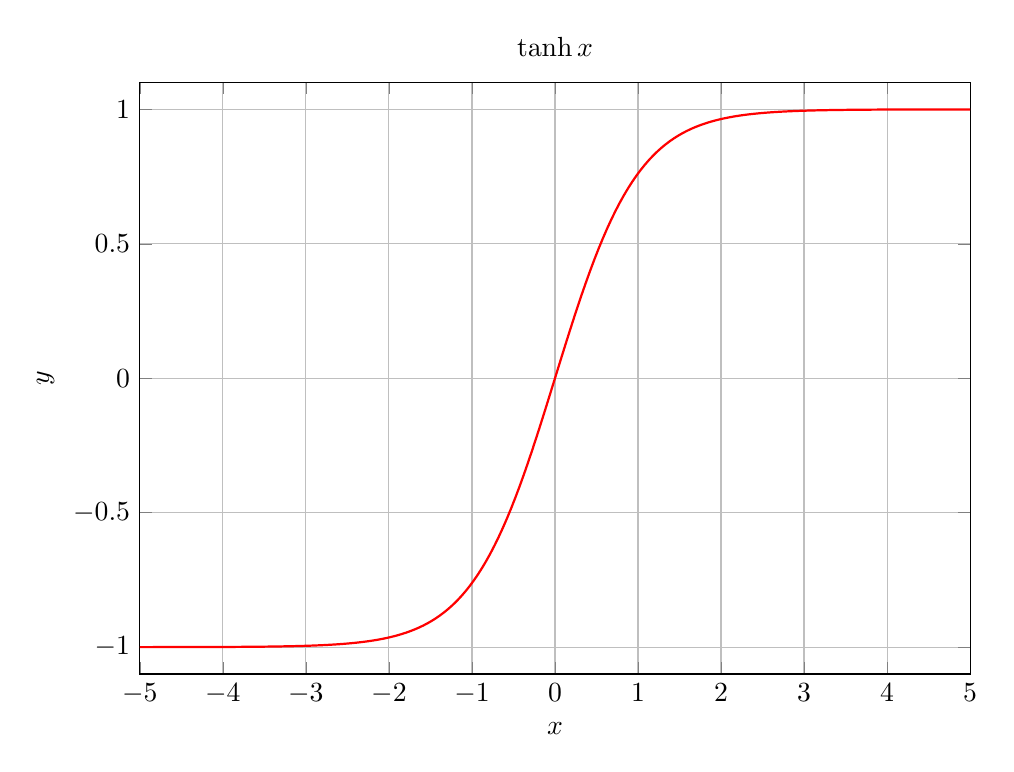
\begin{tikzpicture}
            \begin{axis}[
                title={$\tanh x$},
                xlabel={$x$},
                ylabel={$y$},
                grid=major,
                width=\textwidth,
                height=0.75\textwidth,
                xmin=-5, xmax=5,
                ymin=-1.1, ymax=1.1,
            ]
                \addplot[red, thick, samples=200] {tanh(x)};
            \end{axis}
        \end{tikzpicture}
    \end{minipage}
    \hfill
    \begin{minipage}{0.32\textwidth}
        \centering
        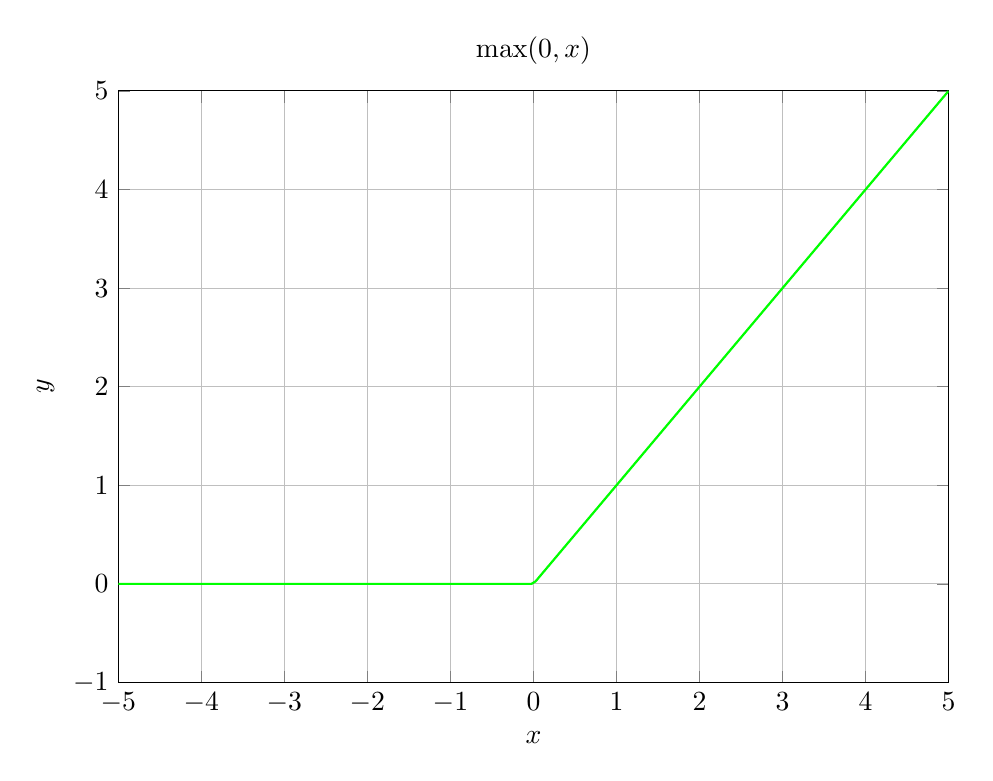
\begin{tikzpicture}
            \begin{axis}[
                title={$\max(0,x)$},
                xlabel={$x$},
                ylabel={$y$},
                grid=major,
                width=\textwidth,
                height=0.75\textwidth,
                xmin=-5, xmax=5,
                ymin=-1, ymax=5,
            ]
                \addplot[green, thick, samples=200, domain=-5:5] {max(0,x)};
            \end{axis}
        \end{tikzpicture}
    \end{minipage}
    \centering
    \caption{Three activation functions.}
\end{figure}

\subsubsection{Loss Function}
\label{sec:loss}

The ultimate purpose of \textit{training} a neural network is to minimise the error between the output predicted by the neural network $\mathbf{\hat{y}}$ and some objective. We typically define this ‘error’ as the loss function $\mathcal{L}: \mathbb{R}^p \times \mathbb{R}^n \to [0, +\infty )$, where $p$ represents the dimension of the parameter vector $\theta$. The loss function is the so-called ‘metric’ that determines the performance of the neural network for any given parameter $\theta$ - minimising the value of $\mathcal{L}(\theta, \mathbf{\hat{y}})$ with respect to $\theta$ is crucial in the optimisation process. As such, the definition of the loss function is an integral step in defining the optimisation problem.

The definition of the loss function usually comprises of some constraints to the model, and how the output of the neural network performs against them. This could take on physical significance, such as in \textit{Physics Informed Neural Networks (PINNs)} where physical constraints naturally arise. In situations where training data with a \textit{ground truth output} is provided, typically defined by $\mathbf{y}$, the loss function is defined to reflect the difference between the predicted output $\mathbf{\hat{y}}$ by the neural network and $\mathbf{y}$.

Of course, the precise definition of the loss function depends on the optimisation problem. For example, a regression problem would employ a loss function different from a classification problem. Even within the class of optimisation problems, different loss functions provide varying perfomances for convergence. We introduce several common loss functions used in regression and classification problems in Table \ref{tab:lfd}, where we define $\mathbf{y} = \left(y_1, \dots, y_n\right)^T$, $\mathbf{\hat{y}} = \left(\hat{y}_1, \dots, \hat{y}_n\right)^T$ and $\epsilon > 0$ for entry 2.
\begin{table}[htbp]
    \centering
    \begin{tabular}{llll}
        \toprule
          & Problem  & Loss Function  &  Definition \\
        \midrule
        1 & Regression       & Absolute Value            & $\frac{1}{n}\sum_{i=1}^n |y_i - \hat{y}_i|$      \\
        2 &Regression       & $\epsilon$-insensitive   & $\frac{1}{n}\sum_{i=1}^n \max{(|y_i - \hat{y}_i| - \epsilon, 0)}$\\
        3 & Regression/Classification       & $L^2$-norm                   & $\frac{1}{n}\sum_{i=1}^n\left(y_i - \hat{y}_i\right)^2$        \\
        4 & Classification  & Hinge                     & $\frac{1}{n}\sum_{i=1}^n\max{(1-y_i\hat{y}_i, 0)}$ \\
        5 & Classification  & Logistic                  & $\frac{1}{n}\sum_{i=1}^n \left(\ln 2\right)^{-1}\ln(1 + e^{-y_i\hat{y}_i})$ \\
        6 & Classification  & Cross-Entropy             & $-\frac{1}{n} \sum_{i=1}^n y_i\ln \hat{y}_i$\\ 
        \bottomrule
    \end{tabular}
    \caption{Commonly used loss functions $\mathcal{L}(\theta, \mathbf{\hat{y}})$ for regression and classification problems. We note that these loss functions assume the availability of training data with outputs $\mathbf{y}$ - in general, not all optimisation problems involving neural networks have access to this and other loss functions are defined to measure a neural network's performance.}
    \label{tab:lfd}
\end{table}

Given the context of optimisation problems, we want to find the optimal value of $\theta$ (which shall be defined as $\hat{\theta}$), giving the global minimum of $\mathcal{L}(\theta, \mathbf{\hat{y}})$. Thus, choosing a loss function that can produce convergence to the global minimum efficiently is of utmost importance. This means that convex functions (which, by definition, can only have one minimum, the global minimum) are generally favoured over non-convex functions, which have multiple (local) minima that an optimisation algorithm might get stuck in. We note that only (6) from Table \ref{tab:lfd} is non-convex, which will require more sophisticated methods to more efficiently locate the global minimum. Such methods are discussed in Section \ref{sec:gd}.

Studies have been conducted to consider the theoretical performances of each of these commonly used loss functions, namely the upper bounds of their rates of convergence (which imply their efficiency). We note that the $L^2$-norm actually has a much slower convergence in both regression and classification problems compared to other convex loss functions discussed \cite{Rosasco2004}.

\subsection{Optimisation Techniques}

Having now introduced the general structure of optimisation problems involving neural networks, we turn our focus towards the optimisation process, in particular, training the neural network and producing the optimum parameters $\hat{\theta}$. This typically involves a method called \textit{gradient descent} that utilises the gradient of $\mathcal{L}$ to iteratively generate stronger approximations of $\theta$. Section \ref{sec:gd} elaborates on this process, while Section \ref{sec:ad} discusses the methods in which gradients can be efficiently and accurately calculated in the context of neural networks.

\subsubsection{Gradient Descent}
\label{sec:gd}

As described in Section \ref{sec:loss}, we want to find the parameters $\theta$ that minimise $\mathcal{L}$. In essence, we want to find $\hat{\theta} = \argmin_\theta \mathcal{L}(\theta, \mathbf{\hat{y}}) $. The most conventional strategy to achieve this is to perform \textit{gradient descent}: that is, to use the gradient of $\mathcal{L}$ with respect to $\theta$ to calculate the next iteration of $\theta$. These new values of the parameters of $\theta$ will then be used to calculate $\mathbf{\hat{y}}$ and therefore the new value of $\mathcal{L}(\theta, \mathbf{\hat{y}})$. This generates a sequence $(\theta_n)_N$, ideally with $N = \infty$, but usually up to some $N$ determined by a stopping condition (typically a hard limit on the number of iterations or when the difference between two consecutive estimates of $\hat{\theta}$ is sufficiently close). 

In order to represent the dependence of a given $\theta_n$, we rewrite the loss function as $\mathcal{L}(\theta,\mathbf{\hat{y}}) = \mathcal{L}(\theta_n, \mathbf{\hat{y}})$. The basic gradient descent method can be described as the following iterative process, given an initial guess $\theta_0$, $\forall n < N$:
$$\theta_{n+1} = \theta_n - \eta \nabla\mathcal{L}(\theta_n, \mathbf{\hat{y}}),$$

where $\nabla\mathcal{L}(\theta_n, \mathbf{\hat{y}})$ is the vector of gradients of $\mathcal{L}$ with respect to each parameter in $\theta_n$, and $\eta$ represents the \textit{learning rate} of the algorithm. This algorithm intuitively makes sense: $\nabla\mathcal{L}(\theta_n, \mathbf{\hat{y}})$ points toward the steepest ascent. By subtracting a multiple of the learning rate from it, we try to find new parameters $\theta_{n+1}$ that give a smaller value of $\mathcal{L}(\theta_n)$ \cite{nazarathy2021}.

There are several conditions on $\eta$ and $\mathcal{L}$ to be fulfilled for the basic gradient descent algorithm to converge to $\hat{\theta}$. In particular, we require that $\nabla\mathcal{L}$ is Lipschitz continuous with constant $L$ and convex for the convergence of $(\theta_n)_\infty$ to $\hat{\theta}$ (the proof of which can be found in Appendix \ref{sec:gdproof}). It is also helpful to have the learning rate $\eta := \frac{1}{L}$, which has a linear convergence at a rate proportional to $\frac{1}{L}$ \cite{gower2015}.

In practice, most loss functions are Lipschitz continuous and convex, and thus the gradient descent algorithm will converge. However, there are several considerations that might affect the effectiveness of the basic gradient descent algorithm:
\begin{enumerate}
    \item In optimisation problems where training data with ground truth outputs are available, if the training data is sufficiently large, the computation of gradients (no matter the algorithm, the most efficient of which are discussed further in \ref{sec:ad} and \ref{sec:contback}) might be too costly. A stronger method of calculating gradients in such a context would be to conduct \textit{stochastic gradient descent} by choosing a random subset of the training data to evaluate in the loss function. We note that each loss function $\mathcal{L}$ can be described as finding the average of the errors of each training point, say $\mathcal{L}(\theta_n,\mathbf{\hat{y}}) = \frac{1}{n} \sum_{i=1}^n l(y_i, \hat{y_i})$. As such, we can think of $\mathcal{L}$ as the expected loss of the function $l$ at each point $i$. Suppose we define some random variable $K$ with $\mathrm{P}(K = j) = \frac{1}{n}$ for $j = 1, ..., n$. It can be easily proven that for any $k \ll n$, we can estimate $\mathcal{L}$ by taking the average of the loss function $g$ at training points $\{y_{K_1}, \dots, y_{K_k}\}$, where $\{K_1, \dots, K_k\}$ are i.i.d. copies of $K$ \cite{kroese2019}. This greatly reduces the computational cost of gradient calculations for gradient descent in particularly large training data.
    
    \item The learning rate $\eta = \frac{1}{L}$ is idealistic in practice. Such a small (and constant) learning rate, while guaranteeing convergence, takes far too long to converge. However, having too large of a learning rate might not allow the sequence $\theta_t$ to converge. As such, more effort is required to calculate the \textit{hyperparameter} $\eta$. There are multiple methods that attempt to remedy this issue. A straightforward method is to decrease the learning rate according to the size of the recalculation of the loss function. Suppose in a certain iteration $\theta_n$, the current learning rate is $\eta = 1$. A possible algorithm is to check whether $\theta_{n+1} = \theta_n - \eta \nabla\mathcal{L}(\theta_n, \mathbf{\hat{y}})$ satisfies $\mathcal{L}(\theta_{n+1}, \mathbf{\hat{y}}) \leq \mathcal{L}(\theta_n)$. If not, this suggests that the current learning rate overcompensates too much - and we can halve the learning rate and check whether the equality is achieved. This reduces the need to calculate a ‘perfect’ constant for $\eta$, instead treating $\eta$ as some function of $t$. Other (more sophisticated) methods include adaptive gradient techniques such as \texttt{AdaGrad}, \texttt{RMSProp} and \texttt{Adam} as found in the \texttt{Flux} package.

    \item As seen in Section \ref{sec:loss}, there exists some non-convex loss functions (such as the commonly used cross-entropy loss function in classification problems). This complicates the gradient descent process, since the choice of starting parameters $\theta_0$ would determine whether the sequence $(\theta_n)_\infty$ would provide a local or global minimum of $\mathcal{L}$. There is a need to ‘escape’ local minima so that the algorithm can give $\hat{\theta}$ as required. The stochastic gradient descent mentioned above actually works to solve this issue: the stochasticity creates \textit{noisy gradients} that helps to nudge $\theta_t$ out of difficult spots \cite{nazarathy2021}.
\end{enumerate}

With all these considerations in mind, a popular choice for gradient descent algorithms is the \textit{Adaptive Moment Estimation} (Adam) algorithm. It makes use of previous gradients in the algorithm to determine the next parameter $\theta_{t+1}$ as well as a separate learning rate for each parameter, scaled to the gradients of the other parameters. With such a combination of methods, it has been empirically the most robust on real datasets \cite{nazarathy2021}.

\subsubsection{Automatic Differentiation and Discrete Backpropagation}
\label{sec:ad}

Having discussed the importance of deriving parameters $\hat{\theta}$ that produce the global minimum of $\mathcal{L}$ through gradient descent, it becomes imperative to use algorithms that derive gradients and derivatives efficiently.

There are a number of methods that do so with varying computational costs. The conventional ideas brought forward by divided differences tend to incur large errors in computation, making gradient calculations inaccurate and thus unreliable. Calculating symbolic expressions of gradients, on the other hand, tends to be rather memory and time consuming \cite{tucker2011}. The computational cost of such a method is further compounded by the fact that functions derived from neural networks tend to be rather complicated in nature. A method that has proven to be time and (relatively) memory efficient is \textit{automatic differentiation} (AD).

There are two distinct types of AD. \textit{Forward-mode AD} computes the derivative of the function along with the function evaluation. A familiar (albeit limited) concept that implements this is the commutative ring of \textit{dual numbers} $\mathbb{D}$ over $\mathbb{R}$ generated by $1$ and $\epsilon$, where $\epsilon^2 = 0$. In the context of neural networks and loss functions, instead of simply evaluating functions with the value of $\theta_n$, evaluating them using dual numbers allows both the solution and its derivative with respect to $\theta_n$. \textit{Reverse-mode AD}, and in particular \textit{backpropagation}, instead evaluates the function first before propagating the derivatives from the output to the input. This section aims to discuss the implementations of backpropagation in the context of a neural network.

Backpropagation can be used to derive the gradients of $\mathcal{L}(\theta, \mathbf{\hat{y}})$ with respect to $\theta$. Suppose that we calculate $\hat{y_i} = g(\theta)$, where $g$ is made up of a composition of $m$ elementary operators $g_1, ..., g_m$. Additionally, suppose that we know the value of $\frac{\partial \mathcal{L}}{\partial \hat{y_i}}$, which we will represent with $\overline{\hat{y_i}}$. These assumptions are valid: First, the functions that define the neural network are (in most circumstances) differentiable. Next, the derivative of the loss function with respect to $\hat{y_i}$ is readily available in practice, as $\mathcal{L}$ is typically explicitly defined and differentiable. This process can be conducted using the following algorithm:
\begin{enumerate}
    \item \textit{Forward Pass.} Evaluate $g$ with the given values of $\theta$, recording the intermediate values after each $g_l$. Thus, we receive a set of values $\{v_1, v_2, \dots, v_m \}$, where $v_m = \hat{y_i}$. These intermediate values (and the functions that connect them) can be represented by a directed acyclic graph (DAG) (an example of which is found in Figure \ref{fig:discretebackprop}) that flows (via the functions $g_l$) from each of the $\theta_j$.
    \item \textit{Chain Rule Application.} By the chain rule, we can easily calculate the values of $\overline{v_l}$, $q = 1, \dots, m$. If $v_l$ contributes directly to some $v_{q}$ via the function $g_q$, then
    $$
    \overline{v_l} = \overline{v_{q}} \cdot \frac{\partial v_{q}}{\partial v_l} = \overline{v_{q}} \cdot \dot{g_q}(v_l).
    $$
    \item \textit{Backward Pass.} Suppose we want to consider the value of $\overline{\theta_j}$. Given $v_p ( = \hat{y_i})$ and $\overline{\hat{y_i}}$, we can work our way up the DAG to $\theta_j$, calculating the intermediate derivatives $\overline{v_q}$ along the way. This can be done for all $\theta_j$.
\end{enumerate}

An example of such an algorithm can be found in Figure \ref{fig:discretebackprop}. Such an algorithm to calculate derivatives only requires a single forward pass and a reverse pass. This means that the algorithm scales well even for more complex models with high dimensional $\theta$ \cite{ketkar2017}.

\begin{figure}[h]\label{discretebackprop}
    \centering
    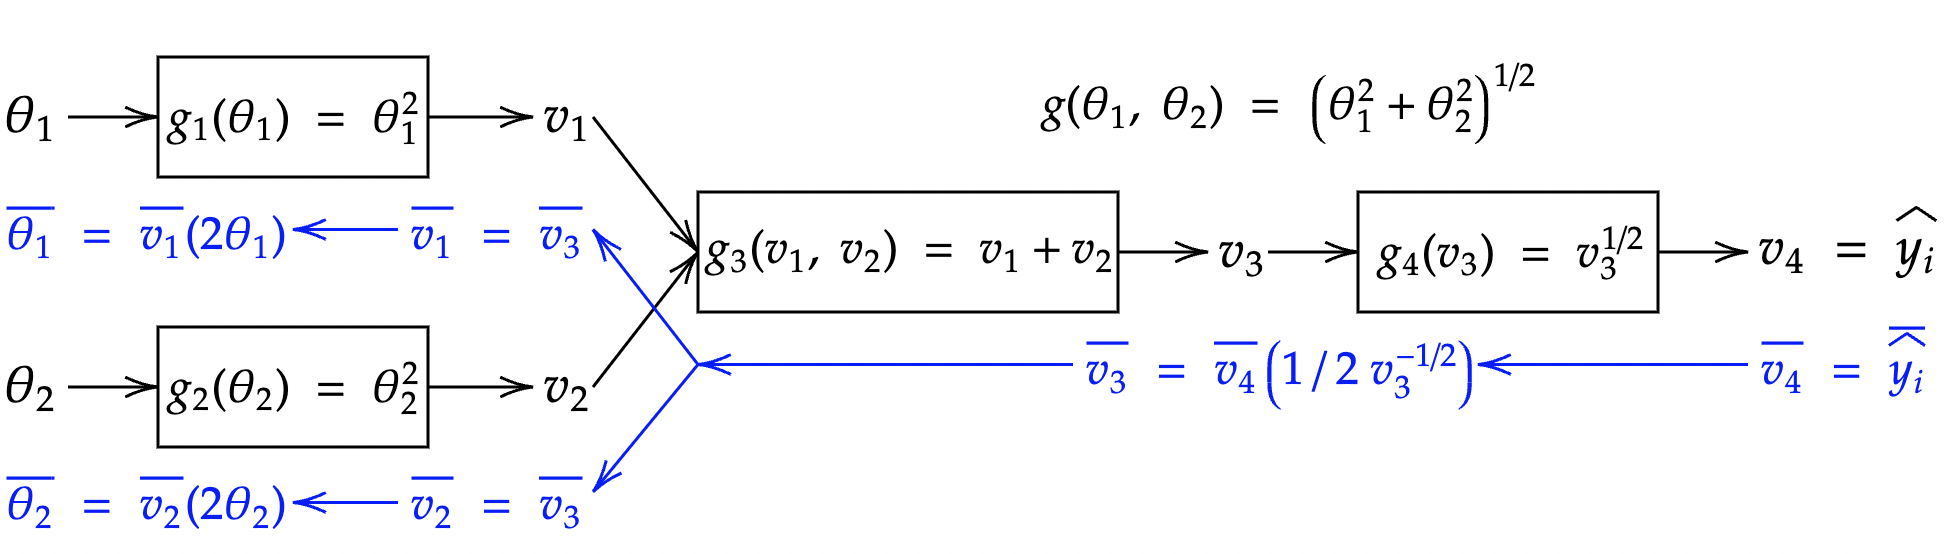
\includegraphics[width=0.8\textwidth]{report/figures/backpropdiscrete.png}
    \caption{A direct acyclic graph representing the intermediate values and the derivatives of $\mathcal{L}$ with respect to each $v_l$. The function used to illustrate this property is $g(\theta_1, \theta_2) = (\theta_1^2 + \theta_2^2)^\frac{1}{2}$. The forward pass is represented in black, while the backward pass is represented in blue.}
    \label{fig:discretebackprop}
\end{figure}

Much work has been put into the improvement of discrete backpropagation algorithms, including the use of Static Single Assignment (SSA) forms to increase efficiency \cite{innes2019}. These advanced implementations of backpropagation can be found in many Julia modules such as \texttt{Zygote}, and we will explore some of them in the following examples in Sections \ref{sec:regex} and \ref{sec:cla}.

\subsection{Example: Regression}
\label{sec:regex}

\textit{Regression} is a technique that approximates data and estimates the relationship between variables. In the context of machine learning, the dependent variable is usually called a \textit{label}. In the second year, we learnt some basics of regression: linear regression in the statistical modelling course and polynomial regression in the numerical analysis course. With the help of neural networks, we might take the idea further and explore non-linear regression. Some of the idea is taken from \cite{SciMLSANUM2024}.

Consider a simple example of a neural network that performs regression based on $y = \sin x$. Assume that we are given $n$ data points between $[-\pi, \pi]$, denoted by $\mathbf{x}$. We try to minimise the difference between the predicted output $f(\mathbf{x})$ and the target output $\sin (\mathbf{x})$, where $f$ is the neural network being considered.

We are now going to present an implementation of this neural network in Julia. We first need to import some packages for later use. 

\begin{verbatim}
using Lux, Random, Optimization, OptimizationOptimisers,
      ComponentArrays, Zygote, Plots, LinearAlgebra
\end{verbatim}

Then we define the data. Let us select 100 evenly spaced points from $[-\pi, \pi]$ and store them in \verb|x|. We will also define the target output in \verb|y|.

\begin{verbatim}
x = range(-pi, pi; length = 100)
y = sin.(x)
\end{verbatim}

To create the neural network model, a Julia package \verb|Lux| is usually used. For the purpose of this example, we could use three layers, all of which are \verb|Dense|, i.e., every neuron in one layer is connected to every other neuron in the next layer. For 100 data points, 10 neurons in the hidden layer would be enough. We can create the composition of such layers using the \verb|Chain| command. The input and hidden layers will have ReLU as the activation function.

\begin{verbatim}
model = Chain(
    Dense(1 => 10, relu),
    Dense(10 => 10, relu),
    Dense(10 => 1)
)
\end{verbatim}

After that, we will implement the loss function based on \verb|norm| from the \verb|LinearAlgebra| package. We might consider our loss function to be the $L^2$-norm of $f(\mathbf{x}) - \sin (\mathbf{x})$, i.e., the square root of the sum of squares of differences between the predicted output and the target output.

\begin{verbatim}
function regression_loss(ps, (model, st, (x, y)))
    return norm(vec(model(x', ps, st)[1]) - y)
end
\end{verbatim}

We now turn our attention to training the neural network. This is essentially equivalent to solving an optimisation problem. We can use \verb|setup| from the package \verb|Lux| to create an initial guess of the parameters and \verb|MersenneTwister| from the package \verb|Random| to make it random.

\begin{verbatim}
ps, st = Lux.setup(MersenneTwister(), model)
\end{verbatim}

To define the optimisation problem, we use the \verb|Optimization| package. Note that we need to wrap \verb|ps| in an array type supplied in the \verb|ComponentArrays| package, as the \verb|Optimization| package requires optimisation to be over an array type. To calculate the gradients needed, \verb|AutoZygote| from the \verb|Zygote| package is used for automatic differentiation. The details will be left to \ref{sec:gd}.

\begin{verbatim}
prob = OptimizationProblem(OptimizationFunction(regression_loss,
       Optimization.AutoZygote()), ComponentArray(ps), (model, st, (x, y)))
\end{verbatim}

To solve the optimisation problem, we use the aforementioned gradient descent method supplied by \verb|Adam| in \verb|OptimizationOptimisers| with appropriate parameters. Again, the details will be left to \ref{sec:gd}.

\begin{verbatim}
ret = solve(prob, Adam(0.03), maxiters = 250)
\end{verbatim}

Lastly, we can visualise our results by plotting supplied in the \verb|Plots| package:

\begin{verbatim}
plot(x, y, label = "Target")
plot!(x, vec(model(x', ret.u, st)[1]), label = "Predicted")
\end{verbatim}

\begin{figure}[htbp]
    \centering
    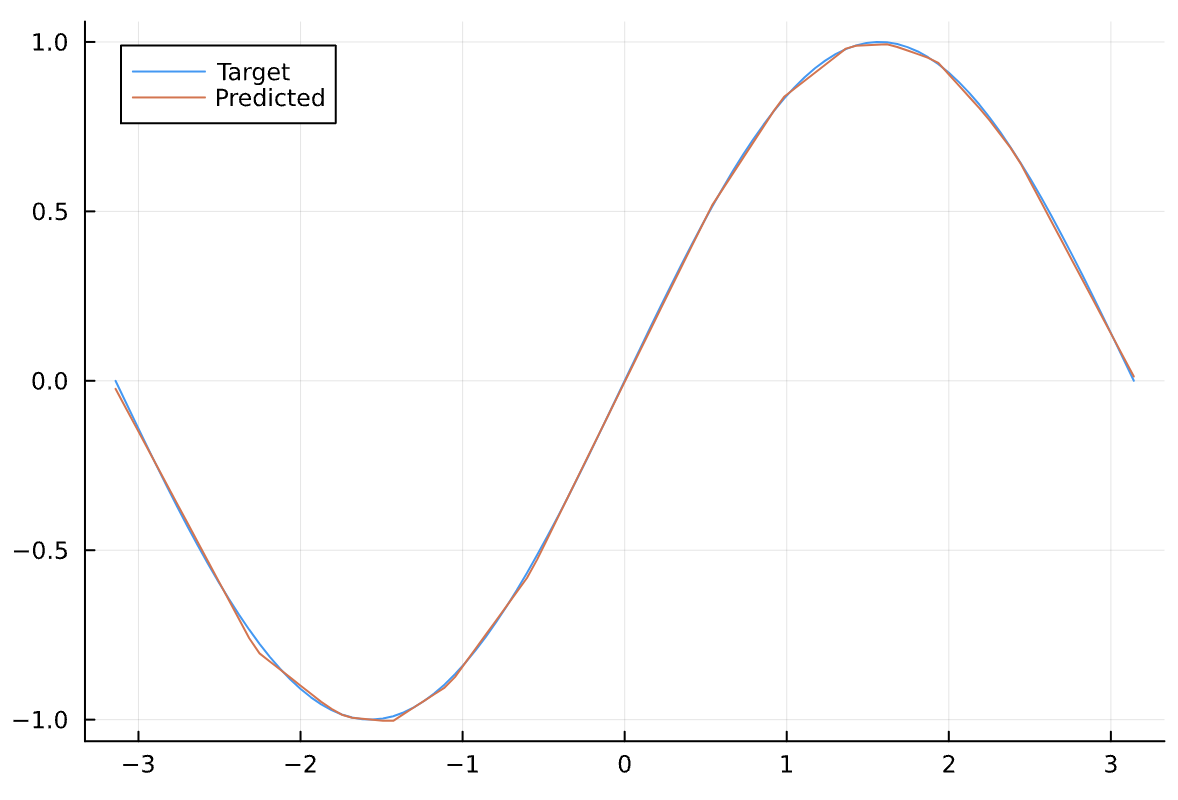
\includegraphics[width=0.8\textwidth]{figures/Regression.png}
    \caption{Regression of $y = \sin x$.}
\end{figure}

This is a pretty impressive result that demonstrates the power of neural networks in terms of regression. However, one disadvantage of neural networks is the model interpretability since understanding the internal workings and the contribution of each feature is difficult. For a simple task like this, this is not a problem; but for a more complex one, this will be a particular drawback.

\subsection{Example: Classification}
\label{sec:cla}

Classification is another application of neural networks. It involves using a neural network to assign labels to input data based on some patterns learnt during the training process. A classic example is digit recognition based on the \textit{Modified National Institute of Standards and Technology database} (MNIST database). This database presents a large collection of handwritten digits given in pixels. The task is to learn from the database and classify the digits. As we can see, it is basically another form of regression; therefore, neural networks would be a suitable model.

We are now going to present a simple implementation of this neural network in Julia. At this point, we will not dive into the details, which will be left to Section \ref{sec:app}. Some of the idea is taken from \cite{Piotr}.

We first need to import some packages for later use. For this task, we introduce another package \verb|Flux|, which is similar to \verb|Lux| mentioned before. We also want to import the MNIST database from the \verb|MLDatasets| package.

\begin{verbatim}
using Flux
using MLDatasets: MNIST
\end{verbatim}

First, we extract data from the database. We split the data into the \textit{training set} and the \textit{test set}, where the former is used to train the model and the latter is used to evaluate its performance on unseen data.

\begin{verbatim}
x_train, y_train = MNIST(split=:train)[:]
x_test, y_test = MNIST(split=:test)[:]
\end{verbatim}

We then need to ‘flatten’ the images so that they become vectors and would be easier to process. For labels, we need to use a technique called \textit{one-hot encoding} to transform categorical variables into \textit{one-hot} form, i.e., a group of bits with one and only one \verb|1| and all other bits \verb|0|.

\begin{verbatim}
x_train_flat = Flux.flatten(x_train)
x_test_flat = Flux.flatten(x_test)
dataset = [(x_train_flat, Flux.onehotbatch(y_train, 0:9))]
\end{verbatim}

After that, we define the neural network for our use. The input layer consists of $28\times 28 = 784$ neurons. We employ two hidden layers, each of which has $1/4$ the number of neurons compared to the previous layer. Finally, the output layer consists of 10 neurons corresponding to the digits 0 to 9. As usual, the ReLU activation function is used.

\begin{verbatim}
model = Chain(
    Dense(784, 196, relu),
    Dense(196, 49, relu),
    Dense(49, 10)
)
\end{verbatim}

The loss function we are using is a modified form of the \textit{cross-entropy}. It measures the performance of a classification model whose output is a probability value between $0$ and $1$. Cross-entropy loss increases as the predicted probability diverges from the actual label.

\begin{verbatim}
loss(x, y) = Flux.Losses.logitcrossentropy(model(x), y)
\end{verbatim}

We are now ready to train our neural network. For this task, it is better to train the neural network several times, or \textit{epochs}. To optimise the performance, we shall use 25 epochs.

\begin{verbatim}
for epoch in 1:25
    Flux.train!(loss, Flux.params(model), dataset, Adam(0.003))
end
\end{verbatim}

By inverting the one-hot encoding using \verb|onecold| and comparing with the target output, we might see the test accuracy given as (where the \verb|+1| is because Julia uses 1-based indexing and \verb|y_test| starts at 0)

\begin{verbatim}
sum(Flux.onecold(model(x_test_flat)) .== (y_test .+ 1)) / length(y_test)
\end{verbatim}

which is normally around $80\%$.  That is great, but not extremely satisfactory. This inspires us to consider a better model, neural differential equations, as detailed below. In Section \ref{sec:app}, we will show that this improves the test accuracy to around $95\%$.

\pagebreak
\section{Neural ODEs}
\label{sec:intro}

\subsection{Motivation}

The method of \textit{neural ODEs} (neural ordinary differential equations) was first proposed in a 2018 paper titled "Neural Ordinary Differential Equations" \cite{chen2018neural}. This paper won the Best Paper Award at NeurIPS in the same year. The inspiration for neural ODEs came from the observation of a specific neural network model called the \textit{residual neural network} (ResNet). This model was introduced by a Microsoft research team in 2015 \cite{he2016deep}. Unlike traditional neural networks, ResNet incorporates residual connections by adding a \textit{residual term} to the output of each layer, as shown in the equation below:
\begin{equation}\label{eq1}
    \textbf{h}_{t+1} = \textbf{h}_t + \sigma\left(\textbf{W}_t\textbf{h}_t + \textbf{b}_t\right).\tag{1}
\end{equation}

The second term in equation \ref{eq1} is in the form of a typical neural network. To obtain the state at layer $t+1$, we perform a calculation using the current state $\textbf{h}_t$, the weight matrix $\textbf{W}_t$ and the bias vector $\textbf{b}_t$ at layer $t$, and an activation function $\sigma$. The first term $\textbf{h}_t$ on the right-hand side of equation \ref{eq1} is the residual term, representing the identity of the hidden state in the layer $t$.
\begin{equation}\label{eq2}
    \textbf{h}_{t+1} = \textbf{h}_t + f\left(\textbf{h}_t, \theta_t\right).\tag{2}
\end{equation}

We can write equation \ref{eq1} in the form of equation \ref{eq2}, where $f$ is a function that depends on the state in layer $t$ and some parameters $\theta_t$ related to this layer. Then, by transforming equation \ref{eq2}, we get
$$\frac{\textbf{h}_{t+1} - \textbf{h}_t}{1}=f\left(\textbf{h}_t, \theta_t\right),$$

which gives
$$\frac{\textbf{h}_{t+\Delta t} - \textbf{h}_t }{\Delta t}\Bigg|_{\Delta t=1}=f\left(\textbf{h}_t, \theta_t\right).$$

Such a form inspires us to make $\Delta t$ infinitesimally small, allowing us to transform this discrete form into a continuous one:
$$\lim_{\Delta t\to 0}\frac{\textbf{h}_{t+\Delta t} - \textbf{h}_t }{\Delta t}= f(\textbf{h}_t, \theta_t,t).$$

This motivates us to consider ordinary differential equations, which can be written as
$$\frac{\mathrm{d}{\textbf{h}}(t)}{\mathrm{d}t}=f(\textbf{h}(t),\theta,t).$$

This is the most important equation in neural ODE. The function $f$ on the right is a function derived from a neural network, with $\theta$ representing the parameters of that network. By convention, since there is no concept of hidden layers in neural ODE, we usually write this function as
$$\dot{z}=f(z(t),\theta,t).$$

\subsection{Comparing Neural ODEs with ResNet}

According to the previous part, we know that the inspiration for neural ODEs originates from ResNet, where it transforms a discrete function into a continuous one. In a ResNet with $L$ layers, the transition between states from one layer to the next is discrete, and each layer has its own function to alter the current state. However, in an ODE network, it defines a continuous vector field which essentially represents a neural network with infinitely many layers. The state change can thus be interpreted as a flow within this vector field.

For neural ODE, we want to solve a problem like this: 

We know (or assume) that our data follow an unknown ODE $\dot{z}=f(z(t),t)$, and we have some observations of the model at time $(t_i)_{i=0,\dots,N}$ along the trajectory; we want to find an approximation $\hat{f}(z(t),\theta,t)$ to the target $f(z(t),t)$.

\begin{figure}[htbp]
    \centering
    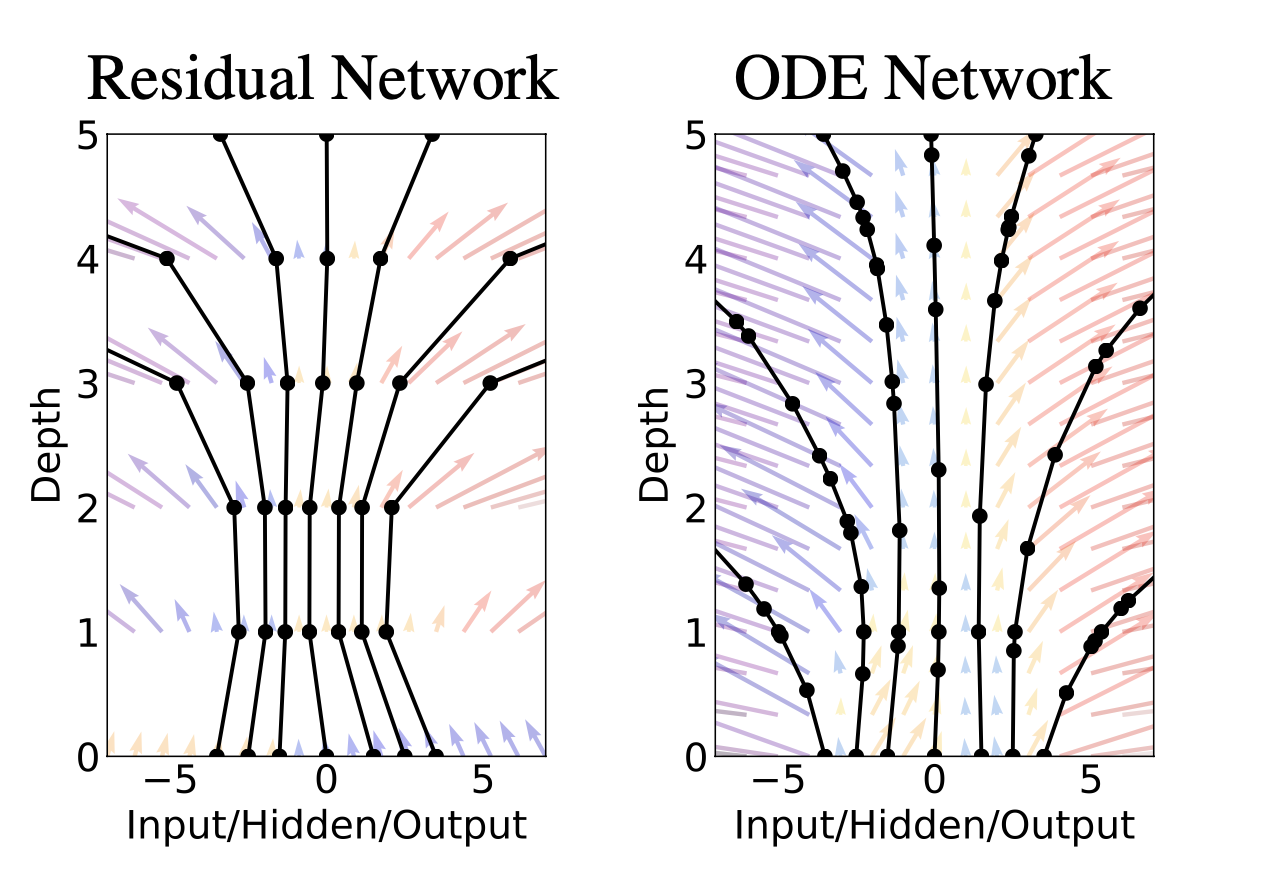
\includegraphics[width=0.5\textwidth]{report/figures/ResNetvsODENet.png}
    \caption{A residual network typically represents discrete transformations, whereas an ODE network defines a continuous vector field. This figure is taken from \cite{chen2018neural}.}
    \label{fig:enter-label}
\end{figure}

Note that the points in the graph on the right-hand side (ODE network) represent the evaluation points. These points can be taken according to an increasing sequence of different time stamps $(t_i)_{i=0,\dots,N}$. Then the values given by the model at those points are $z(t_i)_{i=0,\dots,N}$. They can be obtained by solving an ODE:
$$z(t_i)=\mathrm{ODESolve}(z(t_0),f,t_0,t_i),\quad i=0,\dots,N.$$

Also, the time span for defining a neural ODE would be $[t_0,t_N]$. Since all these points are in the same space, each output has the same dimension as the input vector.

Unlike in neural networks, where depth refers to the number of layers, in neural ODEs, depth can be considered as the number of observation points. For neural networks, more layers can help the model fit the training dataset better in general. Similarly, in neural ODEs, more observation points can provide a better understanding of the $f$ we are looking for, allowing the model to fit the training set better.

\subsection{Various Neural ODE Models}

\subsubsection{Augmented Neural ODEs}

From the previous part, we find that the input space and the output space of a neural ODE always have the same dimension. It poses a problem when simulating certain types of data. For instance, if we want to simulate a sine function, where we want the model to output $\sin x$ for a given input $x$, we might choose to use a simple neural ODE with a one-dimensional input space. In that case, for the sine function, if we input $\frac{\pi}{2}$ and $\frac{3\pi}{2}$, we would expect the model to output $1$ and $-1$, respectively, since the idea of a neural ODE model is to follow a trajectory from the input and try to reach the expected output value after a fixed time. And the function $f$ used to define a neural ODE is Lipschitz continuous, meaning the different trajectories cannot intersect. This makes it difficult for a simple neural ODE to handle such problems.

This is why we sometimes need to use the \textit{augmented neural ODE model}. The idea is to avoid conflicting trajectories by adding more dimensions to the input. In practice, we usually concatenate some zeros to the input and then drop the excess dimensions to the output. This method allows the model to learn a more complex function in a higher-dimension space.

\subsubsection{Neural ODEs with Scientific Machine Learning}

In practice, we sometimes define the function $f$ using a neural network. However, if we have some prior knowledge about the model, we can introduce some interpretable terms to define $f$, and use a neural ODE to approximate the remaining part. This means that we can represent the model as $\dot{z}=g(u,t)+f(u,\theta,t)$, where we already know $g$ (if $g=0$, it is just the simple neural ODE discussed earlier), and we try to approximate $f$ with a neural network. For example, in a Lotka-Volterra system, the dynamic would be
\begin{align*}
    \frac{\mathrm{d}x}{\mathrm{d}t}&=\alpha x-\beta xy,\\
    \frac{\mathrm{d}y}{\mathrm{d}t}&=-\delta y-\gamma xy,
\end{align*}

If we have some information about the model, and we can express it as:
$$
\begin{pmatrix}x'\\ y'
\end{pmatrix}=\begin{pmatrix}\alpha x\\-\delta y\end{pmatrix}+f(x,y),
$$

where $\alpha$ and $\delta$ are known constants and $f$ is an unknown function. Then we can use a neural network only to approximate the function $f$. 

Recent research has shown that integrating information from physical laws and scientific models is particularly useful when there is a limited amount of training data. Additionally, it has the potential to automate the discovery of explicit dynamic equations \cite{rackauckas2020universal}.

\subsubsection{DEFUNCT: Solving Neural ODEs}

\textcolor{red}{There might be some useful parts here for you (Xinyan) to use. Leaving this here for you to think about.}

Consider a neural ODE defined by a neural network $f$. This gives us the differential equation of the system $\dot{z}=f(z(t),\theta,t)$. There are two predominant methods for solving neural ODEs, known as \textit{Discretise-then-Optimise} (DO) and \textit{Optimise-then-Discretise} (OD) \cite{kidger2022neural}.

For now, we introduce the ideas of discretisation and optimisation to provide a general understanding of the techniques required. \textit{Discretisation} (of the neural ODE) involves solving the ODE numerically. These involve breaking the (continuous) differential equation into discrete time steps and employing numerical methods to calculate the solution at each time step. \textit{Optimisation}, on the other hand, involves deriving the parameters $\theta$ that minimise some loss function of our choice.

\subsection{Runge-Kutta Methods}
\label{sec:rungekutta}

Perhaps the most straightforward approach to numerically approximate a solution of ODE $\dot{z}= f(z(t), \theta,t)$, on some interval $\left[a, b\right]$, is to look at the Taylor series expansion of $z$. We first discretise the system and consider the points $t_i = a + ih \in \left[a, b\right]$, where $i = 0, 1, \dots, N - 1$ and $h = \frac{b-a}{N}$. We can therefore use the Taylor series expansion iteratively, centred at each point $t_i$, to find the value of the next point $t_{i + 1}$. This is known as \textit{Euler's method}.

\begin{definition}[Euler's method]
    Given points $t_i = a + ih \in \left[a, b\right]$, $i = 0, 1, \dots, N - 1$, $h = \frac{b-a}{N}$, \textit{Euler's method} is an iterative process to solve the initial value problem $\dot{z}= f(z(t), \theta,t)$, $z(t_0) = z_0$, where
    \begin{align*}
        z(t_0) &= z_0 \\
        z(t_{i+1}) &= z(t_i) + f(z(t_{i}), \theta, t_i)h + O(h^2),\quad\forall i = 1, \dots, N - 1.
    \end{align*}
\end{definition}

The final term in the iterative process is known as the \textit{error term}. We do not include this in the numerical approximation. We note several characteristics of Euler's method:
\begin{itemize}
    \item It is a \textit{first order} approximation, that is, the error of the approximation to the true value is at most linear with respect to $h$. This can be seen from the iterative step as $\frac{z(t_{i+1}) - z(t_i)}{h} = f(z(t_i),\theta,t_i) + O(h)$.
    \item It is a \textit{1-stage} method, in which we only require 1 computation of $f$ at a single point, namely $t_i$ in the iterative step. In a perhaps unintuitive way, we can redefine the iterative step as 
    \begin{align*}
        z(t_{i+1}) &= z(t_i) + h b_1 k_1, \\
        k_1 &= f\left(z(t_i) + h a_{11}k_1, \theta, t_i + hc_1\right),
    \end{align*}
    where $a_{11} = 0, b_1 = 1, c_1 = 0$.
\end{itemize}

These characteristics point toward possible limitations of Euler's method in approximating solutions to initial value problems. The errors of each iterative step can accumulate and result in large errors further away from the initial value. This necessitates having a sufficiently small $h$ for an accurate computation, increasing the computational cost. Furthermore, the assumption of evaluating the derivative (and thus $f$) in the current step $t_i$ might not be an accurate and reliable method to approximate the next step $t_{i+1}$. These limitations call for more robust and computationally efficient algorithms to approximate such solutions. One such class of methods, which extends fairly nicely from Euler's method, are the \textit{Runge-Kutta methods} \cite{sulimayers2003}.

\begin{definition}[Runge-Kutta methods]
    Given points $t_i = a + ih \in \left[a, b\right]$, $i = 0, 1, \dots, N - 1$, $h = \frac{b-a}{N}$, we define an $s$\textit{-stage Runge-Kutta method} that solves the initial value problem $\dot{z}= f(z(t), \theta,t)$, $z(t_0) = z_0$ with iterative step
    \begin{align*}
        z(t_{i+1}) &= z(t_i) + h\sum_{j=1}^s b_j k_j, \\
        k_j &= f\left(z(t_i) + h\sum_{l=1}^s a_{jl}k_l, \theta, t_i + hc_j\right),
    \end{align*}
    where the constants in the matrix/vectors $\mathbf{A} = (a_{jl}), \mathbf{b} = b_j, \mathbf{c} = c_j$ are derived from the Taylor series expansions of $z(t_i)$. These constants are usually represented in a \textit{Butcher's tableau}:
    \begin{equation*}
        \begin{array}{c|ccc}
            c_1 & a_{11} & \cdots & a_{1s} \\
            \vdots & \vdots & \ddots & \vdots  \\
            c_s & a_{s1} & \cdots & a_{ss} \\
            \hline
            & b_1 & \cdots & b_s
        \end{array}
    \end{equation*}
\end{definition}

The Runge-Kutta methods can be categorised into two types: \textit{explicit}, where the matrix $\mathbf{A}$ defined by the Butcher tableau of the method is lower triangular, and \textit{implicit}, where there is no restriction on the structure of the matrix $\mathbf{A}$. The most common example of a higher order Runge-Kutta method is the widely studied \textit{RK4 method} \cite{rungekuttasolvers}. It is a $4$-stage explicit Runge-Kutta method and is a fourth-order approximation. Its Butcher's tableau is specified as
\begin{equation*}
    \begin{array}{c|cccc}
        0  \\
        \frac{1}{2} & \frac{1}{2} \\
        \frac{1}{2} & 0 & \frac{1}{2} \\
        1 & 0 & 0 & 1 \\
        \hline
        & \frac{1}{6} & \frac{1}{3} & \frac{1}{3} & \frac{1}{6} \\
    \end{array}
\end{equation*}

The characteristics specified above make the RK4 method a much stronger algorithm than Euler's method. Given a fixed $h$, while more stages need to be calculated at each iterative step, we note a much better approximation of the solution. Of course, many more sophisticated numerical methods have been developed (such as \texttt{Vern9} \cite{verner2010}) to tackle the approximation of such solutions accurately. These methods give differing levels of accuracy, as seen in Figure \ref{fig:odesolver} (the code for which can be found in Appendix \ref{sec:odesolvecode}), with higher order approximations clearly giving better approximations. Many of these algorithms can be implemented via packages such as \texttt{DifferentialEquations.jl} in Julia.

\begin{figure}
    \centering
    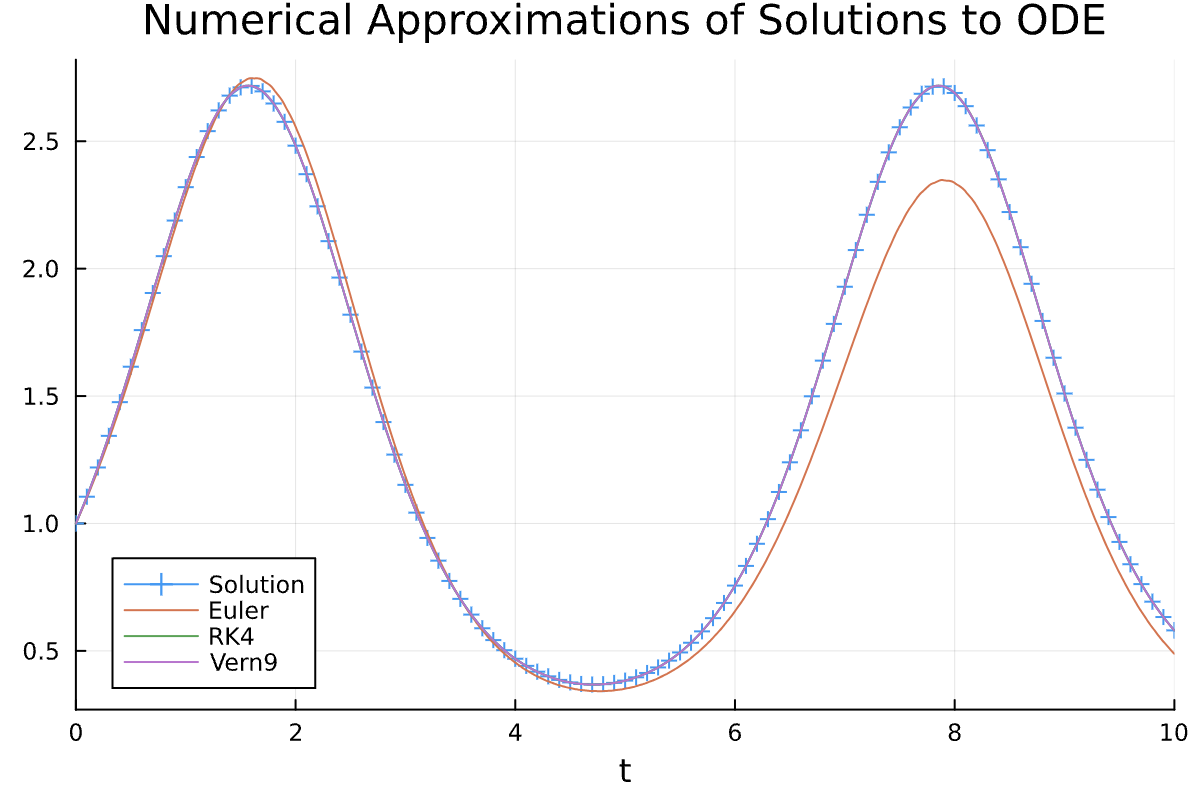
\includegraphics[width=0.6\textwidth]{report/figures/ODESolvers.png}
    \caption{A comparison of ODE Solvers used to solve the initial value problem $\dot{z} = \cos(t)z$, $z(0) = 1$. The errors were calculated by adding the absolute differences of the actual solution and the approximations at discrete times $\{0, 0.1, \dots, 9.9, 10.0\}$.}
    \label{fig:odesolver}
\end{figure}

With such a wide range of numerical methods, there is much consideration in which method is the best. One such consideration is the \textit{absolute stability} of the numerical method. This is an especially important consideration when dealing with stiff ODEs, where the eigenvalues of the linear approximations of $f$ are all negative, with a large ratio between the maximum and minimum real values of the set of eigenvalues. These give rise to numerical instabilities to the numerical methods introduced thus far - essentially requiring an extremely (and thus inefficiently) small value of $h$. A possible alternative to this is to use implicit methods instead. In the context of the Runge-Kutta methods, this means removing the restriction that the matrix $\mathbf{A}$ must be lower triangular. It can be proven that such methods have an \textit{unbounded region of absolute stability}, as compared to explicit Runge-Kutta methods which have \textit{bounded regions of absolute stability} \cite{sulimayers2003}. There is, however, a trade-off in using such implicit methods. The derivation of $k_1, \dots, k_s$ in implicit methods requires solving the $s$ equations simultaneously, instead of in succession as seen in explicit methods. This requires more computational power and might make computation inefficient.

\subsection{Discretise-then-Optimise (DO)}
\label{sec:do}

The Discretise-then-Optimise (DO) method can be described in the following steps:
\begin{enumerate}
    \item \textit{Solve the neural ODE numerically with starting parameters.} This involves choosing an initial ‘guess’ of parameters $\theta$ and solving the neural ODE with the guessed parameters. The Runge-Kutta methods, typically the \texttt{RK4} or \texttt{Vern9} methods as described in Section \ref{sec:rungekutta}, are most commonly used to achieve this.
    \item \textit{Compute the loss function and its gradients with respect to parameters $\theta$.} We can compare the solution derived from the previous step with the dataset. This inevitably gives some amount of discrepancy, which the loss function measures. The calculation of gardients can be achieved through backpropagation as detailed in the next section.
    \item \textit{Perform gradient descent to update the parameters.} This is done using the methods detailed in \ref{sec:gd}, until the loss function is minimised (by monitoring the rate of change of the loss function) or the maximum number of iterations have been reached.
\end{enumerate}

 %Similar to classical neural networks, our objective is to optimise the parameters in the neural ODE model to minimise the loss function. Considering our approximation process as a vector field, we define an increasing time sequence $(t_i)_{i=0,\dots,N}$ for the evaluation points, the value for the evaluation points of a neural ODE model are $z(t_i)_{i=1,\dots,N}$, with:
%$$z(t_i)=\mathrm{ODESolve}(z(t_0),f,\theta(t_0),t_0,t_i),\quad i=0,\dots,N$$

%The loss function would take all the values of the observation points $z(t_i)_{i=0,\dots,N}$, which means that the loss of the model is $\mathcal{L}(z(t_0),z(t_1),\dots,z(t_N))$. The next step is to develop a method to update the parameters in this neural ODE model. It is equivalent to calculate the gradient of the loss function with respect to different parameters, then we can use the gradient to minimise the loss function.

However, the computational cost of backpropagation increases as the number of layers in the neural network increases. This means that performing backpropagation as described above would become computationally expensive. Backpropagating through an ODE solver would also be very inefficient. This motivates us to use a method that calculates gradients without needing to store all the intermediate states while doing backpropagation.

\subsection{Optimise-then-Discretise (OD)}
\label{sec:od}

The Optimise-then-Discretise (OD) method can be described in the following steps. \textcolor{red}{Make sure this is accurate. Think through it properly}:
\begin{enumerate}
    \item \textit{Train $f_\theta$ to provide the parameters of the neural ODE.} This requires the use of a loss function to train the neural network $f_\theta$, providing the parameters required to accurately state the specific ODE in question. Once the parameters have been approximated, we are left with a standard ODE problem.
    \item \textit{Solve the ODE Problem.} As most ODEs do not have analytical solutions, we make use of numerical ODE solvers to approximate the solution of the system.
\end{enumerate}

We note that the OD method does not require an explicit calculation of gradients but instead makes use of the \textit{Adjoint Sensitivity Method}.

\subsubsection{Adjoint Sensitivity Method}

The adjoint sensitivity method was first proposed by Pontryagin in 1962 \cite{pontryagin2018mathematical}. This method provides a way to find the desired gradients by solving another ODE. Consequently, we do not need to store all the activated states for backpropagation, which helps to reduce the computational cost. 

An important point to note is that in the adjoint method we treat $\theta$ as a constant that does not change over time. Therefore, the adjoint method can only be used to solve these specific classes of neural ODEs.

Since there will be $N$ evaluation points and all values at these points contribute to the value of the loss function, we need to obtain the gradient of the parameters with respect to the loss function at each evaluation point; we then aggregate these gradients to get the overall gradient of each parameter for the model. Finally, we update the parameters using this combined gradient.

\subsubsection{Continuous Backpropagation}
\label{sec:contback}

Within the adjoint method, we introduce a quantity $a(t) = \frac{\mathrm{d} \mathcal{L}}{\mathrm{d} z(t)}$, called the \textit{adjoint}. We use this to simplify the process of obtaining the gradients with respect to $z(t)$ and other parameters. Here, we first provide a detailed method for finding the gradient with respect to $z(t)$. We have
\begin{equation}\label{eq3}
    a(t) = \frac{\mathrm{d} \mathcal{L}}{\mathrm{d} z(t)} = \frac{\mathrm{d} \mathcal{L}}{\mathrm{d} z(t+\epsilon)}\frac{\mathrm{d} z(t+\epsilon)}{\mathrm{d} z(t)}=a(t+\epsilon)\frac{\mathrm{d} z(t+\epsilon)}{\mathrm{d} z(t)}. \tag{3}
\end{equation}

Using Taylor expansion to approximate $z(t+\epsilon)$, we have
\begin{equation}\label{eq4}
z(t+\epsilon) = z(t)+\epsilon f(z(t),\theta,t) +\mathcal{O}(\epsilon^2). \tag{4}
\end{equation}

Taking the derivative with respect to $z(t)$ to both sides of (\ref{eq4}) gives
$$
\frac{\mathrm{d}z(t+\epsilon)}{\mathrm{d}z(t)} = \frac{\mathrm{d}z(t)}{\mathrm{d}z(t)}+\epsilon\frac{\mathrm{d}}{\mathrm{d}z(t)}f(z(t),\theta,t)+\mathcal{O}(\epsilon^2).
$$

Here, $\frac{\mathrm{d}z(t)}{\mathrm{d}z(t)}$ equals the identity matrix $\mathbf{I}$ and $\frac{\mathrm{d}}{\mathrm{d}z(t)}f(z(t),\theta,t)$ is the Jacobian matrix of function $f$ with respect to state $z(t)$. This can also be expressed as $\frac{\partial f(z(t),\theta,t)}{\partial z(t)}$.

By combining (\ref{eq3}) to (\ref{eq4}), we can derive the value for $\dot{a}(t)$:
\begin{align}
\dot{a}(t) &= \lim_{\epsilon \to 0^{+}}\frac{a(t+\epsilon)-a(t)}{\epsilon}\notag\\
&=\lim_{\epsilon \to 0^{+}}\frac{a(t+\epsilon)-a(t+\epsilon)\frac{\mathrm{d} z(t+\epsilon)}{\mathrm{d}z(t)}}{\epsilon}\notag\\
&=\lim_{\epsilon \to 0^{+}}\frac{a(t+\epsilon)-a(t+\epsilon)\left(\mathbf{I}+\epsilon\frac{\partial f(z(t),\theta,t)}{\partial z(t)}+\mathcal{O}(\epsilon^2)\right)}{\epsilon}\notag\\
&=\lim_{\epsilon \to 0^{+}}\frac{-\epsilon a(t+\epsilon)\frac{\partial f(z(t),\theta,t)}{\partial z(t)}+\mathcal{O}(\epsilon^2)}{\epsilon}\notag
\\
&=\lim_{\epsilon \to 0^{+}}-a(t+\epsilon)\frac{\partial f(z(t),\theta,t)}{\partial z(t)}+\mathcal{O}(\epsilon)\notag\\
&=-a(t)\frac{\partial f(z(t),\theta,t)}{\partial z(t)}.\notag
\end{align}

Since the loss function is a function of $z(t_i)_{i=1,\dots,N}$, we know the exact value of $a(t)$ at these timestamps when performing backpropagation. These values can be obtained either directly (if the neural ODE is the last layer of the network) or as the results from the backpropagation of the next layer (if the neural ODE layer is in the middle of the network). So we can transform the problem into $N$ initial value problems (IVPs):
\begin{align}{\label{eq5}}
    \dot{a}(t) &= -a(t)\frac{\partial f(z(t),\theta,t)}{\partial z(t)},\notag\\
    a(t_i) &= \frac{\mathrm{d}\mathcal{L}}{\mathrm{d} z(t_i)},\quad i=1,\dots,N. \tag{5}
\end{align}

We can then compute
$$
\frac{\mathrm{d}\mathcal{L}}{\mathrm{d}z(t_{i-1})} =a(t_i)- \int_{t_i}^{t_{i-1}}a(s)\frac{\partial f(z(s),\theta,s)}{\partial z(s)}\mathrm{d}s,\quad i=1,\dots,N.
$$

\subsubsection{Gradients w.r.t. \(\theta\) and \(t\)}

For this part of the proof, we assume that the loss function $\mathcal{L}$ depends only on the final time point $t_N$. If the loss function also depends on intermediate time points $t_1,\dots,t_{N-1}$, we can simply apply the backpropagation using the adjoint method for each interval $[t_{N-1},t_N],\dots,[t_1,t_0]$ in reverse order and sum up the gradients. 

To calculate the gradient with respect to $\theta$ and $t$, similarly, we define two more adjoints as
$$a_{\theta}(t):=\frac{\mathrm{d}\mathcal{L}}{\mathrm{d} \theta},
\quad\quad\quad a_{t}(t):=-\frac{\mathrm{d}\mathcal{L}}{\mathrm{d} t}.$$

(Note that the minus sign in the second term is added to simplify future calculations.)

Using the same method, we can obtain the following two IVPs. For $a_\theta(t)$, to simplify the computation, we assume that $a_\theta(t_N)=0$:
$$
a_{\theta}(t) = \frac{\mathrm{d}\mathcal{L}}{\mathrm{d} z(t)}\frac{\mathrm{d} z(t)}{\mathrm{d}\theta}=a(t)\frac{\mathrm{d} z(t)}{\mathrm{d}\theta}.
$$

Then we have
\begin{align}
\frac{\mathrm{d}\mathcal{L}}{\mathrm{d}\theta}&=\int_{t_0}^{t_N}\frac{\mathrm{d}a(t)}{\mathrm{d}t}\frac{\mathrm{d} z(t)}{\mathrm{d}\theta}+a(t)\frac{\mathrm{d}}{\mathrm{d}\theta}\left(\frac{\mathrm{d}z(t)}{\mathrm{d}t}\right)\mathrm{d}t\notag\\
&=\int_{t_0}^{t_N}\frac{\mathrm{d}a(t)}{\mathrm{d}t}\frac{\mathrm{d}z(t)}{\mathrm{d}\theta}+a(t)\frac{\mathrm{d}f}{\mathrm{d}\theta}\mathrm{d}t\notag\\
&=\int_{t_0}^{t_N}-a(t)\frac{\partial f}{\partial z(t)}\frac{\mathrm{d}z(t)}{\mathrm{d}\theta}+a(t)\left(\frac{\partial f}{\partial z(t)}\frac{\mathrm{d}z(t)}{\mathrm{d}\theta}+\frac{\partial f}{\partial \theta}\right)\mathrm{d}t\notag\\
&=\int_{t_0}^{t_N}a(t)\frac{\partial f}{\partial \theta}\mathrm{d}t\notag\\
&=\int_{t_N}^{t_0}-a(t)\frac{\partial f}{\partial \theta}\mathrm{d}t\notag\\
&=a_{\theta}(t_0)-a_{\theta}(t_N)\notag\\
&=a_{\theta}(t_0).\notag
\end{align}

So we have shown that $a_{\theta}$ is also a function of $t$ such that $$\frac{\mathrm{d}a_{\theta}(t)}{\mathrm{d}t} = -a(t)\frac{\partial f}{\partial \theta}.$$

Then the first initial value problem is 
$$a_\theta(t_N)=0$$
\begin{equation}\label{eq6}
    \frac{\mathrm{d}a_{\theta}(t)}{\mathrm{d}t} = -a(t)\frac{\partial f}{\partial \theta}. \tag{6}
\end{equation}

Next, we consider $a_t(t)$:
$$
a_t(t) = -\frac{\mathrm{d}\mathcal{L}}{\mathrm{d} z(t)}\frac{\mathrm{d} z(t)}{\mathrm{d}t}=-a(t)f(z(t),\theta, t)\implies a_t(t_N) = -a(t_N)f(z(t_N),\theta, t)
$$
\begin{align}
\frac{\mathrm{d}a_t}{\mathrm{d}t}&=-\frac{\mathrm{d}a(t)}{\mathrm{d}t}f(z,\theta,t)-a(t)\left(\frac{\partial f}{\partial z}\frac{\mathrm{d}z}{\mathrm{d}t}+\frac{\partial f}{\partial t}\right)\notag\\
&=a(t)\frac{\partial f}{\partial z}f(z,\theta,t)-a(t)\frac{\partial f}{\partial z}\frac{\mathrm{d}z}{\mathrm{d}t}-a(t)\frac{\partial f}{\partial t}\notag\\
&=-a(t)\frac{\partial f}{\partial t}.\notag
\end{align}

So the second initial value problem is 
$$a_t(t_N)=-a(t)f(z(t),\theta,t)$$
\begin{equation}\label{eq7}
    \frac{\mathrm{d}a_t(t)}{\mathrm{d}t} = -a(t)\frac{\partial f}{\partial t}. \tag{7}
\end{equation}

We noticed that equations (\ref{eq5}), (\ref{eq6}), (\ref{eq7}) follow a similar pattern. By adding a minus sign when defining $a_t(t)$, we ensure that equation (\ref{eq7}) aligns with the pattern of equations (\ref{eq5}), (\ref{eq6}). Accordingly, we define the augumented state $a_{\mathrm{aug}}$ and the corresponding differrential equation $f_{\mathrm{aug}}$ as follows
$$a_{\mathrm{aug}}:= \begin{pmatrix}a\\ a_\theta\\ a_t\end{pmatrix}\quad\quad f_{\mathrm{aug}}\left([z,\theta,t]\right):=\frac{\mathrm{d}}{\mathrm{d}t}\begin{pmatrix}z\\\theta\\ t\end{pmatrix}=\begin{pmatrix}f([z,\theta,t])\\0\\1\end{pmatrix}$$

\[
\frac{\partial f_{\mathrm{aug}}}{\partial (z, \theta, t)} = 
\begin{pmatrix}
\frac{\partial f}{\partial z} & \frac{\partial f}{\partial \theta} & \frac{\partial f}{\partial t} \\
0 & 0 & 0 \\
0 & 0 & 0 
\end{pmatrix}.
\]

This allows us to concatenate all these three adjoints together. Plugging $a_{\mathrm{aug}}$ into (\ref{eq5}), we have
$$
\frac{\mathrm{d}a_{\mathrm{aug}}}{\mathrm{d}t} = -[a(t), a_\theta(t), a_t(t)]\frac{\partial f_{\mathrm{aug}}}{\partial [z,\theta,t]}(t)=-\left[a\frac{\partial f}{\partial z},a\frac{\partial f}{\partial \theta},a\frac{\partial f}{\partial t}\right](t)
$$
$$
a_{\mathrm{aug}}(t_N)=\left[\frac{\mathrm{d}\mathcal{L}}{\mathrm{d} z(t_N)},0,-a(t_N)f(z(t_N),\theta, t_N)\right].
$$

Thus, we only need to solve this initial value problem. By calling the ODE solver on the augmented adjoint once, we are able to calculate all the necessary gradients with respect to $z(t_0)$, $\theta$, $t_0$ and $t_N$.

In Appendix \ref{sec:adjmethod}, we provide a simple example and use the adjoint method to perform backpropagation. A numerical solution is provided to illustrate how this method can be applied.
\textcolor{red}{We might want to write some pros (other than implicitly calculating gradients) and cons for using OD rather than DO.}

\pagebreak
\section{Application: Digit Classifier with Neural ODEs}
\label{sec:app}

In this section, we return our attention to the example we considered in Section \ref{sec:cla}, in which we implemented a digit classifier with around $80\%$ accuracy using classic neural networks. With the help of neural ODEs, we shall implement a better version of this, aiming to boost the test accuracy to approximately $95\%$. The idea is largely taken from Lab 6 of \cite{SciMLSANUM2024}.

To start, we need to import some essential packages. We will use the \verb|DifferentialEquations| and \verb|DiffEqFlux| packages for neural ODEs, and despite the name, \verb|DiffEqFlux| uses \verb|Lux| instead of \verb|Flux|. We also want to load the MNIST database from the \verb|MLDatasets| package, and the \verb|Images| package is useful for plotting images given by pixels.

\begin{verbatim}
using DifferentialEquations, DiffEqFlux, Lux, Random, Optimization,
      OptimizationOptimisers, ComponentArrays, Zygote, Statistics, Images
using MLDatasets: MNIST
imgs, nums = MNIST().features, MNIST().targets
\end{verbatim}

We want to create a neural network with a neural ODE layer to map from an image to a 10-vector where the entry with the largest value is the number itself (plus 1 since Julia indices start from 1), and other entries give us extra information about the chance that it is that number. This reminds us of the one-hot encoding we used before. We can do this with the following function.

\begin{verbatim}
function onehot(nums::AbstractVector)
    n = length(nums)
    ret = zeros(Int, 10, n)
    for j = 1:n
        ret[nums[j]+1, j] = 1
    end
    ret
end
\end{verbatim}

We then ‘flatten’ the images and setup the input layer of the neural network $\mathbb{R}^{28\times28}\rightarrow\mathbb{R}^{20}$. Throughout the neural network, we will use $\tanh$ as the activation function.

\begin{verbatim}
down = Chain(FlattenLayer(), Dense(784, 20, tanh))
rng = MersenneTwister()
down_p, down_st = Lux.setup(rng, down)
\end{verbatim}

The hidden layers $\mathbb{R}^{20}\rightarrow\mathbb{R}^{20}$ are given as a map from initial conditions to final values before passing through the output layer $\mathbb{R}^{20}\rightarrow\mathbb{R}^{10}$ since the output must be a 10-vector. Here, \verb|Tsit5| is a numerical ODE solver which is a modified form of \verb|RK4| mentioned before \cite{TSITOURAS2011770}.

\begin{verbatim}
nn = Chain(Dense(20, 10, tanh), Dense(10, 10, tanh), Dense(10, 20, tanh))
nn_ode = NeuralODE(nn, (0.0f0, 1.0f0), Tsit5(); save_everystep = false,
                   reltol = 1e-3, abstol = 1e-3, save_start = false)
fc = Dense(20, 10)
\end{verbatim}

Now we put everything together, where the \verb|convert| layer maps a solution to an ODE to its final value which we need to wrap in order for it to work with \verb|Lux|.

\begin{verbatim}
m = Chain(; down, nn_ode, convert = WrappedFunction(last), fc)
ps, st = Lux.setup(rng, m)
ps = ComponentArray(ps)
\end{verbatim}

We use the same loss function as before since we simply want to measure that the largest components are in the same spot, not necessarily that the $k^{\mathrm{th}}$ entry is close to $1$ and all other entries are close to $0$.

\begin{verbatim}
logitcrossentropy(ŷ, y) = mean(-sum(y .* logsoftmax(ŷ; dims = 1); dims = 1))
function loss_function(ps, x, y)
    pred, st_ = m(x, ps, st)
    return logitcrossentropy(pred, y), pred
end
\end{verbatim}

After that, we setup the optimisation problem.

\begin{verbatim}
opt_func = OptimizationFunction((ps, _, x, y) -> loss_function(ps, x, y),
                                AutoZygote())
opt_prob = OptimizationProblem(opt_func, ps)
\end{verbatim}

Finally, we prepare data in batches of 100 for efficiency and train the model. We take the last batch as the test set and all the others as the training set.

\begin{verbatim}
const N = 100
M = length(nums) ÷ N - 1
data = [(imgs[:, :, N*(b-1)+1:N*b], onehot(nums[N*(b-1)+1:N*b])) for b = 1:M]
res = solve(opt_prob, Adam(0.003), data)
\end{verbatim}

The test accuracy on the last batch is then given as

\begin{verbatim}
classify(x) = [argmax(x[:,j]) - 1 for j = 1:size(x,2)]
sum(classify(m(imgs[:,:,end-N+1:end], res.u, st)[1]) .== nums[end-N+1:end])/N
\end{verbatim}

which is around $95\%$, a huge improvement!

\pagebreak
\section{Extension: Neural CDEs}
\label{sec:extension}

\subsection{Motivation}

As we have seen before, neural networks and differential equations seem to be irrelevant but, in fact, they have been proven to be two sides of the same coin. In particular, neural ODEs can be seen as a continuous-time analogue to the ResNet. However, there exist certain real-life applications such as time series forecasting where neural ODEs are no longer effective in solving the problem. Fortunately, a British mathematician Terry Lyons developed a novel and exciting field of mathematics, rough path theory, in the 1990s \cite{kidger2022neural}, and we can use some mathematical insights from this theory to develop a new concept called \textit{neural controlled differential equations}.

\subsection{Controlled Differential Equations}

Before defining neural CDEs, it is essential to understand the definition of CDEs. To formally define them, we need to introduce a new notion of integration called \textit{Riemann-Stieltjes integral} and a new concept of real functions called \textit{bounded variation}.

\begin{definition}
    (Riemann-Stieltjes integral) Let $f$ and $g$ be two bounded and real functions defined on $[a,b]$, and let $P=\{a=t_0<t_1<...<t_n=b\}$ be an arbitrary partition on $[a,b]$. $\forall i = 1,...,n$, let $\Delta g_i = g(t_i) - g(t_{i-1})$, $M_i=\mathrm{sup}f(t)$, and $m_i=\mathrm{inf}f(t)$, where $t\in[t_{i-1},t_i]$.
    
    We now define the upper and lower ‘Darboux sums’ similar to those in the construction of Riemann integrals as $U(P,f,g)=\sum M_i\Delta g_i$ and $L(P,f,g)=\sum m_i\Delta g_i$.

    If $\sup L(P,f,g)$ and $\inf U(P,f,g)$ exist and are equal, then denote their common value by $\int^b_af\mathrm{d}g$, or $\int^b_af(t)\mathrm{d}g(t)$, which is the \textit{Riemann-Stieltjes integral} of $f$ with respect to $g$ on $[a,b]$.
\end{definition}

In short, the Riemann-Stieltjes integral is just a simple extension of the Riemann integral.

\begin{definition}
    (Bounded variation) The total variation of a real-valued function $f$ in an interval $[a,b]$, denoted by $V_a^b(f)$, is defined as
$$\sup_{P\in\mathbb{P}}\sum_{i=0}^{n_P-1}\left|f(t_{i+1})-f(t_i)\right|,$$

where $\mathbb{P}=\{P=\{a=t_0<t_1<...<t_{n_P}=b\}\}$, the set of all partitions on $[a,b]$.

Then $f$ is a function of \textit{bounded variation} iff $V_a^b(f)<\infty$.
\end{definition}

\begin{definition}
    (Controlled differential equations (CDEs)) Let $a,b\in\mathbb{R}$ with $a<b$ and let $v,w\in\mathbb{N}$. Let $x:[a,b]\rightarrow\mathbb{R}^v$ be a continuous function of bounded variation. Let $f:\mathbb{R}^w\rightarrow\mathbb{R}^{w\times v}$ be Lipschitz continuous. Let $y_a\in\mathbb{R}^w$.

A continuous function $y:[a,b]\rightarrow\mathbb{R}^w$ is said to be a solution of the following initial value problem:
$$y(a)=y_a, y(t)=y(a)+\int_a^bf(y(s))\mathrm{d}x(s),$$
where $t\in(a,b].$ \cite{kidger2022neural}

In the above controlled integral equation, $\int_a^bf(y(s))\mathrm{d}x(s)$ is a Riemann-Stieltjes integral, and $f(y(s))\mathrm{d}x(s)$ is a matrix vector multiplication.

We can rewrite the above control integral equation as the following control differential equation
$$y(a)=y_a, \mathrm{d}y(t) = f(y(t))\mathrm{d}x(t).$$
\end{definition}

Note that the continuity of $f$ and the bounded variation of $x$ guarantee the existence of the Riemann-Stieltjes integral, and the Lipschitz continuity of $f$ satisfies the condition of the Picard-Lindelöf theorem for controlled differential equations. Hence, the solution to this initial value problem is unique. The existence of the integral and the uniqueness of the solution will not be investigated in detail. For interested readers, see \cite{kidger2022neural} and \cite{rudin1953} for details.

From now on, controlled differential equations will be referred to as CDEs and $y(t)$ will be referred to as $y_t$, which are notations commonly used to describe CDEs.

\subsection{Neural CDEs}

One fundamental assumption of neural CDEs is that the data we observe should form a continuous path $X:[a,b]\rightarrow\mathbb{R}^v$ with bounded variation. This assumption is made simply for theoretical purposes, i.e. the continuous data correspond to an evolutionary process or control path in the neural CDE. However, it is worthwhile to note that it is highly unlikely to observe data in such a form in real-life applications, and thus a trick that converts discrete observations to a continuous control path would be introduced in later parts. Let us now formulate the definition of neural CDEs rigorously, and then it will be clear that neural CDE is the continuous analogue to the recurrent neural network.

\begin{definition}
    (Neural CDEs) Let $f_\theta:\mathbb{R}^w\rightarrow\mathbb{R}^{w\times v}$ be an arbitrary neural network with parameters $\theta$ that represents the dynamics between hidden states. Note that $v$ represents the dimension of the input $X_t$, and $w$ represents the dimension of the hidden states $Z_t$. Let $g_\theta:\mathbb{R}^v\rightarrow\mathbb{R}^w$ be a neural network that maps the input $X_t$ to hidden states $Z_t$.

Then, we define the initial value problem of a neural CDE to be the following
$$Z_a=g_\theta(X_a), Z_t=Z_a+\int_a^tf_\theta(Z_s)\mathrm{d}X_s,$$ where $t\in(a,b],$
or in the differential form
$$Z_a=g_\theta(X_a), \mathrm{d}Z_t=f_\theta(Z_t)\mathrm{d}X_t,$$ where $t\in(a,b].$ \cite{kidger2022neural}
\end{definition}

From the above CDE, we may conclude that the hidden state $Z_t$ of the recurrent neural network can be continuously updated as the input $X_t$ evolves over time. Thus, neural CDE is a continuous analogue of the recurrent neural network. Finally, let $l_\theta:\mathbb{R}^w\rightarrow\mathbb{R}^p$ be a linear map mapping the hidden states $Z_t$ to the output $Y_t$, where $p$ is the dimension of the output $Y_t$. The difference between a neural network and a linear map is that a neural network contains an activation function, and a linear map does not.

\subsection{Solving Neural CDEs}

It is theoretically possible to directly solve a CDE $\mathrm{d}y_t = f(y_t)\mathrm{d}x_t$ with a given initial condition by discretisation. In particular, one could use the following modification of Euler's method to obtain a numerical solution: $y_{i+1}=y_i+f_\theta(y_i)(x(t_{i+1})-x(t_j))$.

CDEs are much harder to solve than ODEs since there is a control term introduced in the equation. For the general case, we do not know whether the control path $x_t$ is differentiable or not. Using powerful tools from rough path theory, one can derive an elegant result called the \textit{log-ODE method}, which approximates the CDE by an ODE containing the log-signature of the control path \cite{morrill2021}. The details of the log-ODE method are omitted here.

Despite the fact that the log-ODE method can be used to solve CDEs under any circumstances, the log-ODE method is quite complicated to be implemented numerically. Fortunately, it can be cleverly avoided in terms of applications. By a standard treatment common in numerical analysis, we can guarantee that the control path $x_t$ is continuously differentiable. We defer the discussion of this technique to later parts of this report. In this case, the CDE can be shown to be equivalent to the following non-autonomous ODE: $\mathrm{d}y_t=g(t,y_t)\mathrm{d}t$, where $g(t,y_t)=f(y_t)\frac{\mathrm{d}x_t}{\mathrm{d}t}$. Then, we can solve this ODE using methods explained in Section \ref{sec:rungekutta} of this report.

Also, note that the backpropagation through CDE is similar to that of ODE. In particular, the discretise-then-optimise method is exactly the same as that of ODE, and the optimise-then-discretise method is similar to that of ODE. Since the proofs are very similar, we omit them here.

\subsection{Application}

It is possible to use neural ODEs to model time series data. However, neural ODEs become less useful when it comes to irregularly sampled time series data. In this final subsection, we propose a naive implementation of using neural CDEs to model financial time series data.

In the context of financial time series, the input data consists of a sequence of discrete data points $\left(t_i,x_i\right)$. As mentioned in the previous subsection, it is possible to construct a continuous control path based on these discrete data points. To do so, we need to employ a standard technique from numerical analysis, called \textit{cubic spline}. 

\subsubsection{Cubic Splines}

In the second-year numerical analysis course, we have learnt about Lagrange basis polynomials and how they can be used to interpolate data. However, when an additional data point is added to the original set of data points, the existing Lagrange polynomials would have to be recalculated. This makes Lagrange basis polynomials computationally inefficient. We seek an alternative set of basis polynomials for interpolation, called \textit{Newton basis polynomials}. The following lemma is not included in \cite{Gautschi2012}, but we state and prove it for completeness.

\begin{lemma}
    Let $n_0(t)=1$, and $\forall j=1,...,k$, let $n_j(t)=\prod_{i=0}^{j-1}(t-t_i)$. Let $P_k$ denote the space of polynomials in $\mathbb{R}$ with  degree less than or equal to $k$. Then $B=\{n_0(t),n_1(t),...,n_k(t)\}$ forms a basis of $P_k$.
\end{lemma}

\begin{proof}
    Since $|B|=k+1=\dim(P_k)$, it suffices to show that $B$ is linearly independent.
    
    We prove by induction on $k\in\mathbb{N}$. The result is trivial for $k=0$. Suppose that the result is true for $k<m$. Then, for $k=m$, suppose that $\exists a_0,a_1,\dots,a_m$ such that $\sum_{i=0}^ma_in_i(t)=0$.

    If $a_0=a_1=\dots=a_m=0$, then $B$ is linearly independent. Otherwise, let $j$ be the largest integer such that $a_j\neq0$. By the induction hypothesis, $\{n_0(t),n_1(t),\dots,n_{j-1}(t)\}$ forms a basis of $P_{j-1}$, and thus $\sum_{i=0}^ma_in_i(t)\neq0$, which is a contradiction. Hence, the result is true for $k=m$.

    By induction, we have that $\forall k\in\mathbb{N}, B=\{n_0(t),n_1(t),\dots,n_k(t)\}$ forms a basis of $P_k$.
\end{proof}

After proving this lemma, we are confident in making the following definitions.

\begin{definition}
    (Newton basis polynomials) Given a sample of $k+1$ data points
$(t_0,x_0), (t_1,x_1), \\\dots, (t_k,x_k)$, the \textit{Newton basis polynomials} corresponding to this sample are defined as $n_0(t)=1$ and $\forall j=1,...,k, n_j(t)=\prod_{i=0}^{j-1}(t-t_i)$.
\end{definition}

\begin{definition}
    (Newton polynomials) Using the same setting as above, we define the \textit{Newton polynomial} that interpolates the sample of data points to be $p_k(t)=\sum_{i=0}^ka_in_i(t)$.
\end{definition}

As the Newton polynomial passes through $(t_0,x_0), (t_1,x_1), \dots, (t_k,x_k)$, the coefficients of the Newton polynomial can be uniquely determined by solving a system of linear equations. The details of this computation are left for the interested readers to check. In other words, given a sample of $k+1$ data points
$(t_0,x_0), (t_1,x_1), \dots, (t_k,x_k)$, the corresponding Newton polynomial is unique.

Since $a_k$ is a linear combination of $x_0,x_1,\dots,x_k$, the coefficients are dependent on $t_0,t_1,\dots,\\t_k$. Let $a_k=[t_0,t_1,\dots,t_k]f$, where $k\in\mathbb{N}$, and $f$ be some unknown function that passes through these points and needs to be estimated using the Newton interpolatory polynomial. The right-hand side is also denoted as the $n^{\mathrm{th}}$ \textit{divided difference} of $f$ relative to $t_0,t_1,\dots,t_k$. The motivation behind this name can be immediately seen from the following lemma.

\begin{lemma}\label{lemma52}
    $\forall k\in\mathbb{N}_{>0}$, we have $$[t_0,t_1,t_2\dots,t_k]f=\frac{[t_1,t_2\dots,t_k]f-[t_0,t_1,\dots,t_{k-1}]f}{t_k-t_0}.$$
\end{lemma}
\begin{proof}
    \cite{Gautschi2012} Let $r(t)=n_{k-1}(f;t_1,t_2,\dots,t_k;t)$ and $s(t)=n_{k-1}(f;t_0,t_1,\dots,t_{k-1};t)$, where $n_{k-1}(f;\\t_1,t_2,\dots,t_k;t)$ means that it is approximating $f$ that passes through $(t_1,x_1), (t_2,x_2), \dots, (t_k,x_k)$, and other Newton basis polynomials are expressed in a similar way.
    
    We claim that
    \begin{equation}\label{eq}
        n_k(f;t_0,t_1,\dots,t_k;t)=r(t)+\frac{t-t_k}{t_k-t_0}(r(t)-s(t)).\tag{*}
    \end{equation}

    By the definition of Newton basis polynomials, it is obvious that the degree of $\mathrm{RHS}$ is less than or equal to $k$. Since Newton interpolatory polynomials are unique, it suffices to show that $\mathrm{RHS}$ passes through $(t_0,x_0), (t_1,x_1), \dots, (t_k,x_k)$.
    
    Substituting $t_0$ into both sides of \ref{eq} gives $\mathrm{LHS}=x_0$ and $\mathrm{RHS}=r(t_0)+\frac{t_0-t_k}{t_k-t_0}(r(t_0)-s(t_0))=s(t_0)=x_0.$

    Substituting $t_k$ into both sides of \ref{eq} gives $\mathrm{LHS}=x_k$ and $\mathrm{RHS}=r(t_k)+\frac{t_k-t_k}{t_k-t_0}(r(t_k)-s(t_k))=r(t_k)=x_k.$

    Substituting $t_i$ into both sides of \ref{eq}, where $i=1,\dots,k-1$, gives $\mathrm{LHS}=x_i$ and $\mathrm{RHS}=r(t_i)+\frac{t_i-t_k}{t_k-t_0}(r(t_i)-s(t_i))=r(t_i)=x_i.$

    In all cases, we have $\mathrm{LHS} = \mathrm{RHS}$, and thus the claim is true.

    Equating the coefficients of both sides of \ref{eq} yields the result.
\end{proof}

Using this result, we can establish a powerful tool called the \textit{table of divided differences}.

\begin{definition}
    (Table of divided differences) Under the same setting as in the previous definition of Newton polynomials, we create a \textit{table of divided differences} as follows:

\begin{center}
\begin{tabular}{ c c c c c }
 $t$ & $f$ & & & \\ 
 $t_0$ & $x_0$ & & & \\  
 $t_1$ & $x_1$ & $[t_0,t_1]f$ & & \\
 $t_2$ & $x_2$ & $[t_1,t_2]f$ & $[t_0,t_1,t_2]f$ & \\
 $t_3$ & $x_3$ & $[t_2,t_3]f$ & $[t_1,t_2,t_3]f$ &  $[t_0,t_1,t_2,t_3]f$ \\
 \dots & \dots & \dots & \dots & \dots
\end{tabular}
\end{center}

where the $i+1^{\mathrm{th}}$ row of the table is defined as 

\begin{center}
\begin{tabular}{ c c c c c c }
$t_i$ & $x_i$ & $[t_{i-1},t_i]f$ & $[t_{i-2},t_{i-1},t_i]f$ & \dots & $[t_0,t_1,\dots,t_i]f.$
\end{tabular}
\end{center}
\end{definition}

The table of divided differences provides a visualisation of the process of computing the coefficients in the Newton polynomial. In particular, the coefficients $a_0,a_1,\dots,a_k$ are the first $k+1$ diagonal entries in the table of divided differences. Using Lemma \ref{lemma52}, one can calculate following this rule: \textbf{Each entry is the difference between the entry immediately to the left and the one above it, divided by the difference between the $t$ value at the right end of the bracket term in this entry and the $t$ value at the left end of the bracket term in this entry}. One can immediately see that the order of the calulation of the coefficients is from the left of the table to the right of it.

\begin{lemma}\label{lemma53}
    $[t_0,t_0,\dots,t_0]f=\frac{1}{k!}f^{(k)}(t_0)$, where the $\mathrm{LHS}$ contains $k+1$ $t_0$'s.
\end{lemma}
\begin{proof}
    \cite{Gautschi2012} Let $s$ be an arbitrary node (a \textit{time point} in the context of time series) not equal to any one of $t_0,t_1,\dots,t_k$.
    
    By the definition of the Newton polynomial, we have
    $$N_{k+1}(f;t_0,t_1,\dots,t_k,s;t)=N_k(f;t)+[t_0,t_1,\dots,t_k,s]f\prod_{i=0}^k(t-t_i).$$
    
    Inserting $t=s$ yields
    $$f(s)=N_k(f;s)+[t_0,t_1,\dots,t_k,s]f\prod_{i=0}^k(s-t_i).$$

    As the choice of $s$ is arbitrary, we can change the notation from $s$ back to $t$, and thus
    $$f(t)-N_k(f;t)=[t_0,t_1,\dots,t_k,s]f\prod_{i=0}^k(t-t_i).$$

    Now we quote without proof a classical result about the error of the interpolation:
    $$f(t)-N_k(f;t)=\frac{f^{(k+1)}(\xi(t))}{(k+1)!}\prod_{i=0}^k(t-t_i),$$
    where $\xi(t)$ is strictly between the smallest and the largest of these nodes.

    Comparing the two results, we have
    $$[t_0,t_1,\dots,t_k,s]f=\frac{f^{(k+1)}(\xi(t))}{(k+1)!}.$$
    
    By letting $t=t_{k+1}$ and replacing $k+1$ by $k$, we obtain
    $$[t_0,t_1,\dots,t_k]f=\frac{1}{k!}f^{(k)}(\xi),$$
    where $\xi$ is defined similarly as before.

    Finally, we let $t_1,\dots,t_k\rightarrow t_0$. Then, by the definition of $\xi$, $\xi\rightarrow t_0$, which yields the result.
\end{proof}

Now we are ready to state and explain the method of cubic spline interpolation formally.

\begin{definition}
    (Cubic splines) Given a sample of $k+1$ data points
$(t_0,x_0), (t_1,x_1), \dots, (t_k,x_k)$, the \textit{cubic spline} $X_t$ corresponding to this sample is an interpolatory curve such that it is twice continuously differentiable.

That is, if $p_i(t)=X(t)|_{[t_i,t_{i+1}]}$, then the following conditions are satisfied:

(1) $p_i(t_i)=x_i, p_i(t_{i+1})=x_{i+1},\quad\forall i=0,1,\dots,k-1;$

(2) $p_i'(t_i)=m_i, p_i'(t_{i+1})=m_{i+1},\quad\forall i=0,1,\dots,k-1;$

(3) $p_{i-1}''(t_i)=p_i''(t_i),\quad\forall i=1,\dots,k-1,$

where $\forall i=0,1,\dots,k$, $m_i$ are chosen constants.
\end{definition}

One might be sceptical about whether condition (3) is necessary, since in time series modelling we would only ensure that the control path $X_t$ is continuously differentiable. However, if condition (3) is dropped, it means that the curvature of the resultant path (which is related to the second derivative of the control path) might not be continuous and thus we believe that there might exist a drastic change in the curvature of the control path which might then lead to unrealistic modelling.

Using the table of divided differences and Lemma \ref{lemma53}, we obtain that the Newton polynomial defined on each time segment $t_i,t_{i+1}$ is
$$p_i(t)=x_i+(t-t_i)m_i+(t-t_i)^2\frac{[t_i,t_{i+1}]f-m_i}{\Delta t_i}+(t-t_i)^2(t-t_{i+1})\frac{m_{i+1}+m_i-2[t_i,t_{i+1}]f}{(\Delta t_i)^2},$$

where $\Delta t_i=t_{i+1}-t_i$.

The above polynomial can be reformulated in terms of a Taylor polynomial:
$$p_i(t)=x_i+m_i(t-t_i)+a_i(t-t_i)^2+b_i(t-t_i)^3,$$

where $\displaystyle a_i=\frac{[t_i,t_{i+1}]f-m_i}{\Delta t_i}-b_i\Delta t_i$ and $\displaystyle b_i=\frac{m_{i+1}+m_i-2[t_i,t_{i+1}]f}{(\Delta t_i)^2}$.

Since $\forall i=1,\dots,k-1, p_{i-1}''(t_i)=p_i''(t_i)$, we have $2a_{i-1}+6b_{i-1}(t_i-t_{i-1})=2a_i$, which simplifies to $a_{i-1}+3b_{i-1}\Delta t_i=a_i$.

Using the coefficients of the Taylor polynomial, we obtain a system of linear equations:
$$\frac{[t_{i-1},t_i]f-m_{i-1}}{\Delta t_{i-1}}+2\frac{m_i+m_{i-1}-2[t_{i-1},t_i]f}{\Delta t_{i-1}}=\frac{[t_i,t_{i+1}]f-m_i}{\Delta t_{i}}-\frac{m_{i+1}+m_{i}-2[t_{i},t_{i+1}]f}{\Delta t_{i}},$$
where $i=1,\dots,k-1$.

Rearranging terms of the above equation yields
$$\Delta t_im_{i-1}+2(\Delta t_{i-1}+\Delta t_i)m_i+\Delta t_{i-1}m_{i+1}=3(\Delta t_i[t_{i-1},t_i]f+\Delta t_{i-1}[t_i,t_{i+1}]f),$$
where $i=1,\dots,k-1$.

There are $k-1$ linear equations with $k+1$ unknowns $m_0,m_1,\dots,m_k$. If $m_0$ and $m_k$ are chosen, the system can then be reduced to a tridiagonal system and thus can be solved using Gaussian elimination.

In terms of applications, the most commonly used cubic spline is the \textit{natural cubic spline}.
\begin{definition}
    (Natural cubic splines) Given a sample of $k+1$ data points
$(t_0,x_0), (t_1,x_1), \\\dots, (t_k,x_k)$, a \textit{natural cubic spline} is a cubic spline $X_t$ such that $X''(t_0)=X''(t_k)=0$.
\end{definition}

Using these additional conditions and the Taylor polynomial, we obtain the following system of linear equations:
$$2\frac{[t_0,t_1]f-m_0-m_1-m_0+2[t_0,t_1]f}{\Delta t_0}=0,$$
$$2\frac{[t_{k-1},t_k]f-m_{k-1}}{\Delta t_{k-1}}+4\frac{m_k+m_{k-1}-2[t_{k-1},t_k]f}{\Delta t_{k-1}}=0,$$

which simplifies to
$$2m_0+m_1=3[t_0,t_1]f,$$
$$m_{k-1}+2m_k=3[t_{k-1},t_k]f.$$

Adding these equations to the system of $k-1$ linear equations, we can readily solve for the constants $m_0,m_1,\dots,m_k$, and thus we can obtain an explicit expression for the control path $X_t$. 

\subsubsection{A Naive Implementation}

In this section, we propose a naive implementation of neural CDEs to model irregularly sampled time series data.

\textbf{Description of the time series data:}

The time series data used are adapted from kaggle. It records the daily adjusted closing price of Amazon from 15/05/1997 to 02/08/2017 excluding holidays, which is reasonable since the stock market is closed during holidays. Hence, it is an irregularly sampled time series.

\textbf{Data preprocessing:}

The data preprocessing process contains several steps. Firstly, the time series data are normalised using min-max scaling. In particular, the time series data are now set to be in the range $[0,1]$ using the formula $p_i=\frac{x_i-x_{\min}}{x_{\max}-x_{\min}}$. Secondly, all dates are reorganised into the unified format "yyyy/mm/dd". Then, we transform each date into the relative date, which is the difference in days between the initial date and itself. Finally, we use the time series data of the form $(t_i,x_i)$, where $t_i\in\mathbb{N}, x_i\in[0,1]$ to create a natural cubic spline. The relevant codes are included in Appendix \ref{sec:datatime}.

\textbf{Training:}

In this part, we will only give a brief overview of the training process.

Recall that the entire forecasting process consists of three linear maps. In particular, $g_\theta:\mathbb{R}^v\rightarrow\mathbb{R}^w$ is a neural network that maps the input $X_t$ to hidden states $Z_t$, $f_\theta:\mathbb{R}^w\rightarrow\mathbb{R}^{w\times v}$ is an arbitrary neural network with parameters $\theta$ that represents the dynamics between hidden states. Note that $v$ represents the dimension of the input $X_t$, and $w$ represents the dimension of the hidden states $Z_t$. Finally, $l_\theta:\mathbb{R}^w\rightarrow\mathbb{R}^p$ is a linear map that maps the hidden states $Z_t$ to the output $Y_t$, where $p$ is the dimension of the output $Y_t$.

The main goal is to find the optimal parameters for each of the neural networks and the final linear map. In the training process of the second neural network, we need to incorporate the derivative of the control path obtained in the previous section into the CDE. In other words, use the method mentioned previously to convert the neural CDE to an ODE.

There exist online Python libraries that uses neural CDEs to achieve time series forecasting. See \cite{Jhin2023} for details.

\pagebreak
\section{Conclusion}

In this report, we began with neural networks and their applications. We then developed a powerful tool called neural differential equations. After exploring their properties and highlighting their connection with residual networks, we carried on our work and delved into how they could be solved using numerical methods. Our report culminated with a classic application, the MNIST digit classifier. Furthermore, we discussed neural CDEs as a useful extension to neural ODEs. The field of scientific machine learning is a highly active one, attracting scientists and mathematicians alike. Various libraries are being developed, the most important of which in Julia is the \hyperlink{https://sciml.ai/}{\texttt{SciML}} package.

\section*{Acknowledgments}
\addcontentsline{toc}{section}{Acknowledgement}

We would like to thank Dr. Olver, our project supervisor, and his PhD students Mr. VandenHeuvel and Mr. Pu for their continued support and guidance throughout the project. Also, we would like to thank Dr. Salvi and Prof. Cass for kindly sharing their lecture notes which inspire the neural CDE extension section in this report.

\pagebreak
\appendix
\section{Comparison of ODE Solvers}
\label{sec:odesolvecode}

In this appendix, we provide the Julia code used to compare several numerical ODE solvers, namely the \texttt{Euler()}, \texttt{RK4()} and \texttt{Vern9()} methods. The code can also be found in the project's GitHub repository \citationneeded, with file name \texttt{ODE\_Solvers.ipynb}. The initial value problem evaluated here was $\dot{z} = \cos(t)z, z(0) = 1$ in the interval $[0.0, 10.0]$, which has a trivial solution $z(t) = e^{\sin t}$. We first import relevant packages and define the problem in Julia:
\begin{verbatim}
using DifferentialEquations, Plots
function ode_problem!(dz, z, p, t)
    dz[1] = cos(t) * z[1]
end
u0 = [1.0]
T = 10.0
tspan = (0.0, T)
prob = ODEProblem(ode_problem!, u0, tspan)
\end{verbatim}

We then generate the solutions for each method by discretising the interval and applying the relevant method:
\begin{verbatim}
times = 0:0.1:T
euler = solve(prob, Euler(), tstops=times)
rk4 = solve(prob, RK4(), tstops=times)
vern9 = solve(prob, Vern9(), tstops=times)
\end{verbatim}

The additional code below is used to generate Figure \ref{fig:odesolver}, comparing the actual solution with the approximations provided by the numerical ODE solvers. We note that \texttt{rk4} and \texttt{vern9} produce outputs that do not give the solution at the specified output points (namely \texttt{times}), requiring an extra step each to discretise:
\begin{verbatim}
actualsol = exp.(sin.(times))
plot(times, actualsol, marker=:+, label="Solution", 
    title="Numerical Approximations of Solutions to ODE")
plot!(euler, label="Euler")
rk4_discrete = [rk4(time)[1] for time in times]
plot!(times, rk4_discrete, marker=:"circle", markersize=:2, label="RK4")
vern9_discrete = [vern9(time)[1] for time in times]
plot!(times, vern9_discrete, label="Vern9")
\end{verbatim}

\pagebreak
\section{Proof of Convergence of Gradient Descent Algorithm}
\label{sec:gdproof}

In this appendix, we prove the convergence of the gradient descent algorithm (as presented in Section \ref{sec:gd}) that generates the sequence $(\theta_n)_\infty$, taking similar ideas from \cite{gower2015}.

We first note that since $\mathbf{\hat{y}}$ depends on the values of $\theta$, we can simply consider a univariate function $\mathcal{L}(\theta)$. We can thus define the concepts of $L$-Lipschitz continuity and convexity:

\begin{definition}[$L$-Lipschitz continuity]
    A function $f$ is $L$\textit{-Lipschitz continuous} in interval $\Theta \subset \mathbb{R}^p$ if $\exists L > 0$, $\forall \theta_x, \theta_y \in \Theta$, we have
    $$
    \|f(\theta_x) - f(\theta_y)\| < L \| \theta_x - \theta_y\|
    $$
\end{definition}

\begin{definition}[$L$-smoothness]
    A function $f$ is $L$\textit{-smooth} if $\nabla f$ is $L$-Lipschitz continuous.
\end{definition}

\begin{definition}[Convexity]
    A function $f$ is \textit{convex} on $\mathbb{R}^p$ if $\forall \theta_x, \theta_y \in \mathbb{R}^p$, $\forall t \in [0, 1]$, we have
    $$
    f(t\theta_x + (1 - t)\theta_y) \leq tf(\theta_x) + (1-t)f(\theta_y).
    $$
\end{definition}

In order to prove the convergence of the gradient descent algorithm, we need two lemmas:

\begin{lemma}
    If $\mathcal{L}$ is $L$-smooth, then the following inequalities hold $\forall  \theta_x \in \mathbb{R}^p$: 
    \begin{align}
        \mathcal{L}(\theta_x - \frac{1}{L}\nabla \mathcal{L}(\theta_x)) - \mathcal{L}(\theta_x) &\leq -\frac{1}{2L} \| \nabla \mathcal{L}(\theta_x)\|_2^2, \label{B1} \\
        \mathcal{L}(\hat{\theta}) - \mathcal{L}(\theta_x) &\leq -\frac{1}{2L}\|\nabla \mathcal{L}(\theta_x)\|_2^2. \label{B2}
    \end{align}
\end{lemma}
\begin{proof}
    We note that
    \begin{align*}
        \mathcal{L}(\theta_x - \frac{1}{L}\nabla \mathcal{L}(\theta_x)) &\leq \mathcal{L}(\theta_x) - \frac{1}{L} \langle\nabla \mathcal{L}(\theta_x), \nabla \mathcal{L}(\theta_x)\rangle + \frac{L}{2} \|\frac{1}{L}\nabla \mathcal{L}(\theta_x) \|_2^2 \\
        &= \mathcal{L}(\theta_x) - \frac{1}{2L}\| \nabla \mathcal{L}(\theta_x)\|_2^2
    \end{align*}
    by $L$-smoothness, giving (\ref{B1}). We note that for (\ref{B2}), $\mathcal{L}(\theta_x) \geq \mathcal{L}(\hat{\theta}) \ \forall \theta_x$. This completes the proof.
\end{proof}

\begin{lemma}
    If $\mathcal{L}$ is convex and $L$-smooth, then
    \begin{align}
        \mathcal{L}(\theta_y) - \mathcal{L}(\theta_x) &\leq \langle \nabla \mathcal{L}(\theta_y), \theta_y - \theta_x \rangle - \frac{1}{2L} \|\nabla \mathcal{L}(\theta_y) - \nabla \mathcal{L}(\theta_x) \|_2^2, \label{B3} \\
        \langle \nabla \mathcal{L}(\theta_y) - \nabla \mathcal{L}(\theta_x), \theta_y - \theta_x \rangle &\geq \frac{1}{L} \|\nabla \mathcal{L}(\theta_y) - \nabla \mathcal{L}(\theta_x). \| \label{B4}
    \end{align}
\end{lemma}
\begin{proof}
    (\ref{B3}) can be proven by stating
    \begin{align*}
        \mathcal{L}(\theta_y) - \mathcal{L}(\theta_x) &= \mathcal{L}(\theta_y) - \mathcal{L}(\theta_z) + \mathcal{L}(\theta_z) -\mathcal{L}(\theta_x) \\
        &\leq \langle \nabla \mathcal{L}(\theta_y), \theta_y - \theta_z \rangle + \langle \nabla \mathcal{L}(\theta_x), \theta_z - \theta_x \rangle + \frac{L}{2} \|\theta_z - \theta_x\|_2^2
    \end{align*}
    by convexity and $L$-smoothness. We can minimise $\theta_z = \theta_x - \frac{1}{L}(\nabla \mathcal{L}(\theta_x) - \nabla \mathcal{L}(\theta_y))$, which gives
    \begin{align*}
        \mathcal{L}(\theta_y) - \mathcal{L}(\theta_x) &\leq \langle \nabla \mathcal{L}(\theta_y), \theta_y - \theta_x \rangle - \frac{1}{L} \|\nabla \mathcal{L}(\theta_y) - \nabla \mathcal{L}(\theta_x) \|_2^2 + \frac{1}{2L} \|\nabla \mathcal{L}(\theta_y) - \nabla \mathcal{L}(\theta_x) \|_2^2 \\
        &= \langle \nabla \mathcal{L}(\theta_y), \theta_y - \theta_x \rangle - \frac{1}{2L} \|\nabla \mathcal{L}(\theta_y) - \nabla \mathcal{L}(\theta_x) \|_2^2.
    \end{align*}
    Finally, (\ref{B4}) follows since $\theta_x$ and $\theta_y$ are interchangeable, and adding up both versions of (\ref{B3}) gives the inequality
    $$
    0 \leq \langle \nabla \mathcal{L}(\theta_y) - \nabla \mathcal{L}(\theta_x), \theta_y - \theta_x \rangle - \frac{1}{L} \|\nabla \mathcal{L}(\theta_y) - \nabla \mathcal{L}(\theta_x) \|.
    $$
\end{proof}

We thus require that $\mathcal{L}(\theta, \mathbf{\hat{y}})$ is $L$-smooth and that $\mathcal{L}$ is convex for the gradient descent algorithm to produce a convergent sequence $(\theta_n)_\infty$ to $\hat{\theta} = \arg\min_\theta \mathcal{L}(\theta, \mathbf{\hat{y}})$:

\begin{theorem}[Convergence of Gradient Descent Algorithm]
    Let $\mathcal{L}$ be $L$-smooth and let $\theta_n$ for $n = 1, \dots$ be the sequence of iterates generated by the gradient descent algorithm
    $$
    \theta_{n+1} = \theta_{n} - \eta \nabla \mathcal{L}(\theta_n)
    $$
    It follows that the sequence $(\theta_n)_\infty$ is convergent to $\hat{\theta}$, where $\hat{\theta} = \argmin_\theta \mathcal{L}(\theta)$.
\end{theorem}
\begin{proof}
    Since $\mathcal{L}$ is convex and $L$-smooth, and by (\ref{B4}),
    \begin{align*}
        \|\theta_{t+1} - \hat{\theta}\|_2^2 &= \|\theta_{t} - \hat{\theta} - \eta \nabla \mathcal{L}(\theta_t)\|_2^2 \\
        &= \|\theta_{t} - \hat{\theta}\|_2^2 - \frac{2}{L}\langle \theta_t - \hat{\theta}, \nabla \mathcal{L}(\theta_t)\rangle + \frac{1}{L^2}\|\nabla \mathcal{L}(\theta_t)\|_2^2 \\
        &\leq \| \theta_t - \hat{\theta}\|_2^2 - \frac{1}{L^2}\|\nabla \mathcal{L}(\theta_t)\|_2^2.
    \end{align*}
    
    We see that $(\|\theta_t - \hat{\theta}\|_2^2)_\infty$ is a decreasing sequence in $t$ (which already means it is convergent). By (\ref{B1}), we have that
    \begin{equation}
    \mathcal{L}(\theta_{t+1}) - \mathcal{L}(\theta_t) \leq \mathcal{L}(\theta_t) - \mathcal{L}(\hat{\theta}) - \frac{1}{2L}\|\nabla \mathcal{L}(\theta_t) \|_2^2. \label{B5}
    \end{equation}
    
    Applying convexity, we have that
    \begin{align*}
        \mathcal{L}(\theta_t) - \mathcal{L}(\hat{\theta}) &\leq \langle \nabla \mathcal{L}(\theta_t), \theta_t - \hat{\theta} \rangle \\
        &\leq \| \nabla \mathcal{L}(\theta_t)\|_2 \| \theta_t - \hat{\theta} \| \\
        &\leq \| \nabla \mathcal{L}(\theta_t)\|_2 \| \theta_1 - \hat{\theta} \|.
    \end{align*}
    
    Combining the above statement with (\ref{B5}) gives
    \begin{equation}
        \mathcal{L}(\theta_{t+1}) - \mathcal{L}(\theta_{t}) \leq \mathcal{L}(\theta_{t}) - \mathcal{L}(\hat{\theta}) - \frac{1}{2L} \frac{1}{\| \theta_1 - \hat{\theta} \|^2}\left(\mathcal{L}(\theta_t) - \mathcal{L}(\hat{\theta})\right)^2. \label{B6}
    \end{equation}
    
    We define $\delta_t = \mathcal{L}(\theta_{t}) - \mathcal{L}(\hat{\theta})$, $\beta = \frac{1}{2L} \frac{1}{\| \theta_1 - \hat{\theta} \|^2}$, and manipulating (\ref{B6}) gives:
    \begin{align*}
        \delta_{t+1} &\leq \delta_t - \beta \delta_t^2 \\
        \beta \frac{\delta_t}{\delta_{t+1}} &\leq \frac{1}{\delta_{t+1}} - \frac{1}{\delta_{t}} \\
        \beta &\leq \frac{1}{\delta_{t+1}} - \frac{1}{\delta_{t}}.
    \end{align*}
    
    Summing both sides over $t = 1, ..., n - 1$ gives 
    $$
    (n-1)\beta \leq \frac{1}{\delta_n} - \frac{1}{\delta_1} \leq \frac{1}{\delta_n}.
    $$
    
    This means that for any given $n$,
    \begin{equation}
        \mathcal{L}(\theta_n) - \mathcal{L}(\hat{\theta}) \leq \frac{2L\|\theta_1 - \hat{\theta}\|^2}{n-1},
    \end{equation}
    
    which means that for any arbitrarily small $\epsilon > 0$, we can find $N$ sufficiently large, such that $\forall n > N$, $|\mathcal{L}(\theta_n) - \mathcal{L}(\hat{\theta})| < \epsilon$. This concludes the proof.
\end{proof}

\pagebreak
\section{A Simple Example of the Adjoint Method}
\label{sec:adjmethod}

In this appendix, we provide a simple example and try to apply the adjoint method to find the desired gradients. We aim to create a model where, given an input $x$, the output is $x\mathrm{e}$. We initialise our neural ODE with $f(z(t),\theta,t)=\theta z$, or $\dot{z}=\theta z$ over the timespan $[t_0,t_1]$, where $\theta$, $t_0$, $t_1$ are constants. Since $f$ is autonomous, we can fix $t_0 = 0$, and only make $t_1$ a trainable time parameter. Suppose that the model has one evaluation point at time $t_1$. Given an input $x$, the output will be $x\mathrm{e}^{\theta t_1}$. So, the model will perfectly align with our goal if $\theta t_1=1$.

After setting up the model, we provide one training data as $z(t_0)$. We can then solve the initial value problem and get $z(t) = z(t_0)\mathrm{e}^{\theta(t-t_0)}$, then output $z(t_1)=z(t_0)\mathrm{e}^{\theta t_1}$. We also provide the expected output value $c:=z(t_0)\mathrm{e}$.
To use the adjoint method, we first calculate the loss function. For simplicity, we choose the mean square error (MSE) as the loss function. Thus, we have
$$\mathcal{L} = \frac{1}{2}\left(c-z(t_0)\mathrm{e}^{\theta t_1}\right)^2.$$

Here we add $\frac{1}{2}$ to simplify the derivatives.
For the adjoint method, we need to calculate the derivative for $a_{\mathrm{aug}}$ and its derivative $\frac{\mathrm{d}a_{\mathrm{aug}}}{\mathrm{d}t}$. To make it clear, in this example, instead of solving an IVP for $a_{\mathrm{aug}}$ in one call, we will solve three IVPs with respect to $a$, $a_\theta$, and $a_t$ numerically, providing an idea of how this method actually works.

For $a$, we know $$\frac{\mathrm{d}{a}}{\mathrm{d}{t}}=-a\frac{\partial f(z(t),\theta,t)}{\partial z(t)}=-a\theta,\quad\quad a^{\mathrm{initial}} = z(t_1)-c.$$

Solving this IVP, we get $$a(t)= (z(t_1)-c)\mathrm{e}^{-\theta(t-t_1)}.$$

Next, for $a_\theta$, $$\frac{\mathrm{d}{a_\theta}}{\mathrm{d}{t}}=-a\frac{\partial f(z(t),\theta,t)}{\partial \theta}=-az,\quad\quad a^{\mathrm{initial}}_\theta=0.$$

So we have
\begin{align}
\frac{\mathrm{d}{a_\theta}}{\mathrm{d}{t}}&=-a(t)z(t)\notag\\
&= -(z(t_1)-c)\mathrm{e}^{-\theta(t-t_1)}z(t_0)\mathrm{e}^{\theta t}\notag\\
&= -(z(t_1)-c)z(t_0)\mathrm{e}^{\theta t_1}.\notag
\end{align}

Here, $c_\theta:=-\frac{\mathrm{d}{a_\theta}}{\mathrm{d}{t}}$ is a constant. Hence, $a_\theta(t_0) =\frac{\mathrm{d}L}{\mathrm{d}\theta} =t_1c_\theta$, and this is the gradient we need for updating $\theta$.

For $a_t$,
$$
\frac{\mathrm{d}{a_t}}{\mathrm{d}{t}}=-a\frac{\partial f(z(t),\theta,t)}{\partial t}=0,
$$
\begin{align}
a^{\mathrm{initial}}_t &= -a(t_1)f(z(t_1),\theta,t)\notag\\
&=-a(t_1)z(t_1)\theta\notag\\
&=-(z(t_1)-c)z(t_1)\theta.\notag
\end{align}

So we can obtain the required gradients to update the time parameter $\frac{\mathrm{d}L}{\mathrm{d}t_1}=(z(t_1)-c)z(t_1)\theta$.

After obtaining these gradients, we can use them in the gradient descent to adjust the parameters in the model. Additionally, by setting some random values for $\theta$ and $t_1$, we can see that the gradients we get always point in the right direction to make $t_1\theta$ closer to $1$.

\pagebreak
\section{Data Preprocessing of Financial Time Series}
\label{sec:datatime}

In this appendix, we provide the Julia code used to preprocess the financial time series.

We first read the data into the compiler.
\begin{verbatim}
using DataFrames, CSV, Plots
amzn = CSV.read("/Users/tianshiliu/Desktop/financial time series
folder/data/AMZN.csv",DataFrame)
\end{verbatim}

We plot the original data to obtain a visualisation of the discrete time series data.
\begin{verbatim}
p1 = plot(amzn."Date", amzn."Adj Close", title="Original Time Series
Data", legend=:topright)
\end{verbatim}

Having observed the pattern of the data, we find that the trend of the daily adjusted closing price of Amazon is overall increasing. Thus, the best strategy to scale the data is to use min-max scaling as explained previously.
\begin{verbatim}
using Statistics
function min_max_scaling(column)
    min_val = minimum(column)
    max_val = maximum(column)
    return (column .- min_val) ./ (max_val .- min_val)
end
amzn_norm = copy(amzn)
for col in names(amzn_norm)
    if eltype(amzn_norm[!, col]) <: Number
        amzn_norm[!, col] = min_max_scaling(amzn_norm[!, col])
    end
end
\end{verbatim}

We then have to calculate the relative dates as defined in the last section of the report.

The first step is to extract the sorted dates and adjusted close values. 
\begin{verbatim}
using Dates
dates = amzn_norm."Date"
print(dates)
adj_close = amzn_norm."Adj Close"
\end{verbatim}

Next, we transform the dates into the desired format "yyyy/mm/dd".
\begin{verbatim}
output_date_format = DateFormat("yyyy/mm/dd")
function parse_mixed_date(date_str)
    date_parsed = nothing
    try
        date_parsed = Date(date_str, DateFormat("m/d/yyyy"))
    catch
    end
    if isnothing(date_parsed)
        try
            date_parsed = Date(date_str, DateFormat("m/dd/yyyy"))
        catch
        end
    end
    return date_parsed
end
formatted_dates = [Dates.format(parse_mixed_date(date), 
    output_date_format) for date in dates]
\end{verbatim}

Finally, we can calculate the relative dates.
\begin{verbatim}
Formatted_dates = Date.(formatted_dates, output_date_format)
init_date = Formatted_dates[1]
rel_dates = []
for x in Formatted_dates
    x = x - init_date
    push!(rel_dates, Dates.value(x))
end
\end{verbatim}

The last step is to create a cubic spline using the processed time series data.
\begin{verbatim}
using DataInterpolations
time_series = collect(zip(rel_dates, adj_close))
cubic_spline_t = DataInterpolations.CubicSpline(rel_dates, rel_dates)
cubic_spline_p = DataInterpolations.CubicSpline(adj_close, rel_dates)
function cubic_spline(t)
    return (cubic_spline_t(t), cubic_spline_p(t))
end
\end{verbatim}
\pagebreak
\bibliography{bibliography.bib}
\end{document}